\documentclass[a4paper, 12pt,oneside]{book}
% \documentclass[a4paper, 12pt,times,numbered,print,index,oneside]{book}
\usepackage[utf8]{inputenc}
\usepackage{graphicx}
\usepackage{listings}
\usepackage{color}
\usepackage{booktabs}
\usepackage{tabularx}
% \usepackage{subfigure}
\usepackage{afterpage}
\usepackage{amsmath,amssymb}            
\usepackage{rotating}
\usepackage{fancyhdr}
\usepackage{xcolor}
\usepackage{eurosym}
\usepackage{pdflscape}
\usepackage{tabu}
\usepackage{geometry}
\usepackage{float}
\usepackage{bbm}
\usepackage{bm}
\usepackage[scriptsize]{caption}
\usepackage{subcaption}
\usepackage{multirow}

\usepackage[citestyle=authoryear,bibstyle=numeric,backend=biber,maxcitenames=1,minbibnames=99, maxbibnames=100]{biblatex}

% mie
\usepackage{enumitem}

\hyphenation{a-gen-tiz-za-zio-ne}

\addbibresource{Bibl.bib}

\newcommand{\sign}{\text{sign}}
\usepackage{amsfonts, mathrsfs, comment, amsthm,epsfig,epstopdf,titling,url,array}
\usepackage{algorithm}
\usepackage{algpseudocode}
\renewcommand{\thealgorithm}{\thechapter.\arabic{algorithm}}
% \usepackage{algorithmic}

% rename require ensure in input output
% \floatname{algorithm}{Procedure}
\algrenewcommand{\algorithmicrequire}{\textbf{Input:}}
\algrenewcommand{\algorithmicensure}{\textbf{Output:}}
\newcommand{\Initialize}{\textbf{Initialize:}}


% \usepackage{algorithm2e}
%\usepackage[linesnumbered,ruled]{algorithm2e}

\providecommand{\keywords}[1]
{
  \small	
  \textbf{Keywords:} #1
}
\providecommand{\parolechiave}[1]
{
  \small	
  \textbf{Parole Chiave:} #1
}

\graphicspath{{pictures/}}

% Custom colors
\definecolor{clr-background}{RGB}{255,255,255}
\definecolor{clr-text}{RGB}{0,0,0}
\definecolor{clr-string}{RGB}{163,21,21}
\definecolor{clr-namespace}{RGB}{0,0,0}
\definecolor{clr-preprocessor}{RGB}{128,128,128}
\definecolor{clr-keyword}{RGB}{0,0,255}
\definecolor{clr-type}{RGB}{43,145,175}
\definecolor{clr-variable}{RGB}{0,0,0}
\definecolor{clr-constant}{RGB}{111,0,138} % macro color
\definecolor{clr-comment}{RGB}{0,128,0}
\definecolor{deepblue}{rgb}{0.45,0.95,0.36}
\definecolor{deepred}{rgb}{0,0,0}
\definecolor{deepgreen}{rgb}{0.67,0.31,0.31}
\definecolor{deepblack}{rgb}{0.11,0.11,0.11}
\definecolor{lightblue}{rgb}{0.77, 0.89, 0.93}
\definecolor{codeblack}{rgb}{0.20,0.20,0.20}
\definecolor{codered}{rgb}{1,0.6,0.6}
\definecolor{codelightblue}{rgb}{0.6,0.6,0.6}
\definecolor{codegray}{rgb}{0.5,0.5,0.5}

\newcommand\cppstyle{\lstset {
    language=C++,
    backgroundcolor=\color{codeblack},
	basicstyle=\scriptsize\ttfamily\color{white},
	keywordstyle=\scriptsize\ttfamily\color{clr-type},
	stringstyle=\scriptsize\ttfamily\color{red},
	commentstyle=\scriptsize\ttfamily\color{green},
	morecomment=[l][\color{magenta}]{\#},
	numbers=left,
	numberstyle=\ttfamily\color{codegray},
	stepnumber=1
}}

% Python for external files
\newcommand\cppexternal[2][]{{
		\cppstyle
		\lstinputlisting[#1]{#2}}}

%\setlength{\paperwidth}{16cm}
%\setlength{\paperheight}{24cm}
%\setlength{\oddsidemargin} {2. cm}
%\setlength{\evensidemargin} {2. cm}
%\addtolength{\oddsidemargin} {-0.4 cm}
%\addtolength{\evensidemargin} {-0.4 cm}


\linespread{1.1}
\usepackage{csquotes}
\usepackage[italian]{babel}
%\usepackage[latin1]{inputenc}
%\renewcommand{\captionfont}{\normalfont \sffamily \itshape \small}
\renewcommand*\contentsname{Summary}
\newtheorem{theorem}{Theorem}[section]
\usepackage[hidelinks]{hyperref}

\usepackage{bm}
\usepackage{mymacros}

\renewcommand\lstlistingname{Code}
\renewcommand\lstlistlistingname{Codes}

\makeatletter
\gdef\lst@numberfirstlinefalse{\global\let\lst@ifnumberfirstline\iffalse}
\lst@AddToHook{Init}{\global\let\lst@ifnumberfirstline\iftrue}
\makeatother


\theoremstyle{definition}
\newtheorem{defn}{Definition}[section]
\newtheorem{conj}{Conjecture}[section]
\newtheorem{exmp}{Example}[section]

\theoremstyle{plain}
\newtheorem{lem}[thm]{Lemma}
\newtheorem*{cor}{Corollary}

\theoremstyle{remark}
\newtheorem*{rem}{Remark}
\newtheorem*{note}{Note}

\pagestyle{empty}

\emergencystretch=1em

\renewcommand*{\bibfont}{\normalfont\small}

\begin{document}
\thispagestyle{empty}
%\begin{titlepage}
\vspace*{-1.5cm} \bfseries{
\begin{center}
    {{\Large{\textsc{Alma Mater Studiorum $\cdot$ Università di
    Bologna}}}}
	\rule[0.1cm]{15.8cm}{0.1mm}
    \rule[0.5cm]{15.8cm}{0.6mm}
    {\normalsize{\textsc { Scuola di Ingegneria e Architettura\\
    \vspace{5mm}
    Dipartimento di Informatica - Scienza e Ingegneria -\\
    \vspace{5mm}
    Corso di Laurea Magistrale in Ingegneria Informatica}}}\\
	\vspace{10mm}
	{\small{\sc Anno Accademico 2021/2022}}%inserire l'anno accademico a cui si è iscritti
\end{center}
\vspace{10mm}
\begin{center}
    {\LARGE\textbf{- RELAZIONE FINALE -}}\\
    \vspace{3mm}
    {\LARGE\textbf{ANALISI DI BATTISTRADA}}\\
    \vspace{3mm}
    {\LARGE\textbf{TRAMITE L'UTILIZZO DEL}}\\
    \vspace{3mm}
    {\LARGE{\bf PROFILOMETRO LASER GOCATOR}}\\
    \vspace{10mm} {\large{\sc Esame di Computer Vision and Image Processing M}}
\end{center}
\vfill
\par
\noindent
\begin{minipage}[t]{0.47\textwidth}
    {\large{\sc Autore:}\\
    {\bf \textsc{Gabriele Tornatore}}}\\
\end{minipage}
\vspace{20mm}
}\thispagestyle{empty} \vspace*{.75truecm} \normalfont \cleardoublepage

%\include{dedica}\thispagestyle{empty} \vspace*{.75truecm} \cleardoublepage

\pagenumbering{roman}

\tableofcontents\addcontentsline{toc}{chapter}{Indice}\label{contents}
\thispagestyle{empty} \vspace*{.75truecm} \cleardoublepage

\listoffigures\thispagestyle{empty}\addcontentsline{toc}{chapter}{Elenco delle figure}\vspace*{.75truecm} \cleardoublepage

%\listofalgorithms\thispagestyle{empty}\addcontentsline{toc}{chapter}{List of Algorithms} \vspace*{.75truecm} \normalfont \cleardoublepage

%\include{Sommario}\thispagestyle{empty} \vspace*{.75truecm} \cleardoublepage

%\include{abstract}\thispagestyle{empty} \vspace*{.75truecm} \cleardoublepage

\pagestyle{plain}\renewcommand{\chaptermark}[1]{\markboth{\chaptername\ \thechapter.\ #1}{}} 
\renewcommand{\sectionmark}[1]{\markright{\thesection.\ #1}}         
% \fancyhead[LE,RO]{\bfseries\thepage}    
                                        
% \fancyhead[RE]{\bfseries\leftmark}    
% \fancyhead[LO]{\bfseries\rightmark}     
\renewcommand{\headrulewidth}{0.3pt} 

\pagenumbering{arabic}
\chapter{Introduzione}
\label{Cha:introduzione}
\thispagestyle{empty}

Viviamo in un mondo 3D con processi di produzione che richiedono un'ispezione delle parti, ad alta velocità, altamente accurata. Le soluzioni di visione artificiale progettate per supportare la produzione automatizzata possono essere complicate da progettare, configurare e installare, e spesso richiedono personale specializzato con un background ingegneristico.\\
\newline
Le soluzioni 2D progettate per risolvere i problemi di misurazione 3D sono complicate, costose e spesso non hanno successo. Il 2D, semplicemente, non può compensare la variazione di altezza senza una sorta di compromesso in termini di costi, qualità o affidabilità.\\
\newline
Sebbene le soluzioni 3D siano tradizionalmente considerate costose o complicate da configurare, la rivoluzionaria famiglia di prodotti Gocator di LMI semplifica la misurazione 3D per l'automazione in fabbrica.\\
\newline
LMI Technologies Inc. (LMI) è leader mondiale nella tecnologia dei sensori smart 3D per applicazioni di ispezione e di misura in ambito industriale ma non solo; LMI sviluppa costantemente nuove soluzioni 3D che consentono agli utenti finali di sfruttare gli enormi vantaggi della tecnologia laser applicata al controllo di qualità, all'ottimizzazione dei materiali per ridurre gli sprechi oppure all'automazione nelle moderne realtà industriali, al fine di migliorarne la produttività.\\
\newline
Il progetto ha l'obiettivo di interfacciarsi con il Gocator e di creare una demo per \textit{PC}, comprensiva di \textit{GUI}, che permette l'elaborazione della \textit{point cloud}, effettuando misurazioni sui prodotti presi in esame.\\
\newline
Il tutto è stato svolto presso il T3LAB (Technology Transfer Team), un consorzio senza fini di lucro espressamente ideato per realizzare il trasferimento tecnologico tra realtà accademica e aziendale, per influenzarne reciprocamente saperi e strategie.\\

\noindent La relazione è articolata come segue:
\begin{itemize}
	\item nel \textbf{capitolo \ref{Cha:gocator}} viene presentato il gocator e il settaggio utilizzato;
	\item nel \textbf{capitolo \ref{Cha:analisi}} vengono descritti i prodotti presi in analisi e gli algoritmi utilizzati;
	\item nel \textbf{capitolo \ref{Cha:desktop}} viene presentato lo sviluppo dell'applicazione desktop e le sue funzionalità;
	\item il \textbf{capitolo \ref{Cha:conclusioni}} conclude la relazione presentando i risultati ottenuti, gli obiettivi raggiunti ed eventuali problematiche che potrebbero essere risolte in futuro;
\end{itemize}
Il codice e l'applicazione dell'intero progetto possono essere reperiti nella seguente repository git: \href{https://github.com/it9tst/computer-vision}{https://github.com/it9tst/computer-vision}
\cleardoublepage
\chapter{Gocator}
\label{Cha:gocator}
\thispagestyle{empty}

Il Gocator è un sistema di visione 3D che cattura la forma e la posizione di un oggetto, indipendentemente dal colore della superficie e senza opportune calibrazioni.\\
\newline
Il design semplice e flessibile del Gocator consente alle fabbriche di ridurre i costi e massimizzare la redditività migliorando l'efficienza nella convalida dei prodotti. Esso riesce a supportare le richieste di misure 3D accurate, dalle aziende, in settori quali: fusione di alluminio, gomma e produzione di pneumatici, lavorazione del legno, assemblaggio di automobili, food \& packaging, medicale ecc..\\

\begin{figure}[H]
	\centering
	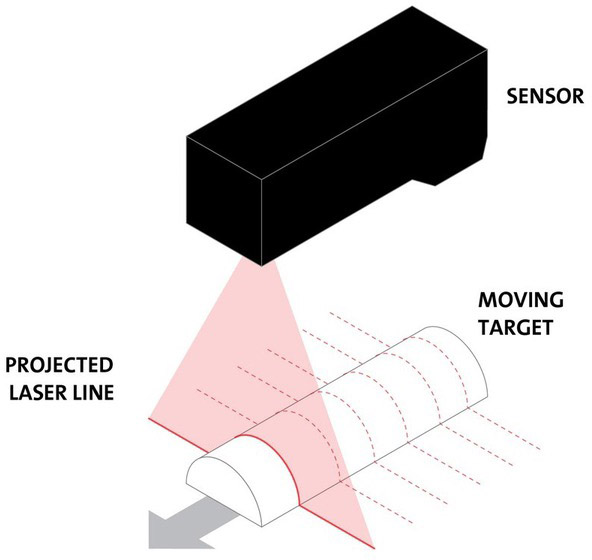
\includegraphics[scale=0.30]{./pictures/gocator_1.jpg}
	\caption{Funzionamento di un profilometro laser.}\label{fig:gocator_1}
\end{figure}

\newpage

\noindent Il modello che è stato utilizzato per l'esecuzione del progetto è il Gocator 2350, facente parte della serie 2300, disponibile in cinque modelli standard, che hanno come caratteristiche comuni:

\begin{itemize}
	\item \textbf{Risoluzione megapixel:} 1280 punti per risoluzione del profilo;
	\item \textbf{Campo visivo:} fino a 1260 mm;
	\item \textbf{Campo di misura:} fino a 800 mm;
\end{itemize}

\ \\
\noindent In particolare, il modello 2350 presenta le seguenti caratteristiche: 

\begin{itemize}
	\item \textbf{Risoluzione dell'asse X:} 0.150 mm;
	\item \textbf{Risoluzione dell'asse Z:} 0.019 mm;
	\item \textbf{Campo visivo (FOV):} 158 mm - 365 mm;
	\item \textbf{Distanza minima (CD):} 300 mm;
	\item \textbf{Campo di misura (MR):} 400 mm;
\end{itemize}

\begin{figure}[H]
	\centering
	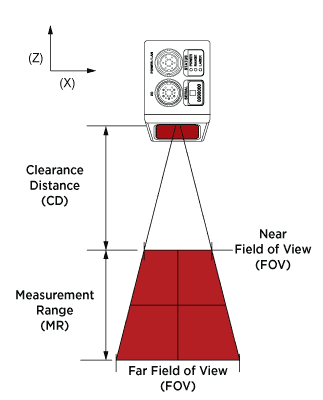
\includegraphics[scale=0.60]{./pictures/gocator_2.png}
	\caption{Caratteristiche visive del Gocator.}\label{fig:gocator_2}
\end{figure}

\section{Settaggi}
Il collegamento tra il sensore e il PC avviene tramite cavo Ethernet, quindi è importante conoscere l'indirizzo IP del Gocator. Una volta identificato l'indirizzo IP, basta inserirlo nel browser web per interagire con l'interfaccia web che LMI mette a disposizione dell'utente.\\
\newline
Per i nostri propositi sono stati modificati alcuni settaggi che rimarranno immutati anche durante le scansioni, mentre i settaggi che potrebbe essere utile modificare in \textit{runtime}, si troveranno anche nella nostra applicazione.

\subsection{Area Attiva}
L'area attiva si riferisce alla regione all'interno del massimo campo visivo del sensore, utilizzata per la profilatura laser (figura \ref{fig:active_area}). Riducendo l'area attiva, il sensore può funzionare a velocità più elevate.\\
\newline
Per i nostri scopi, è stata scelta una dimensione di area attiva di:

\begin{itemize}
	\item \textbf{X Field of View:} 300 mm;
	\item \textbf{Measurement Range:} 250 mm;
\end{itemize}

\begin{figure}[H]
	\centering
	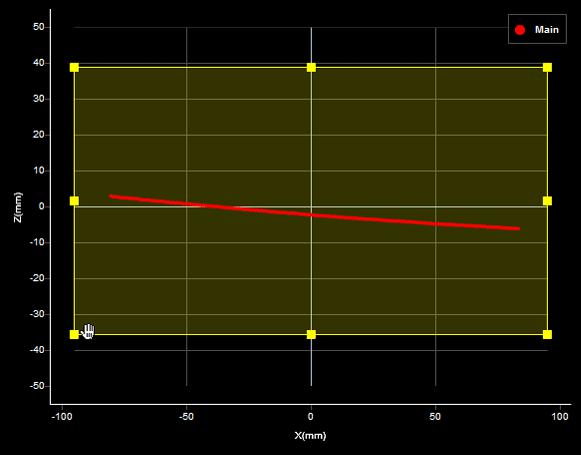
\includegraphics[width=0.7\columnwidth]{./pictures/active_area.png}
	\caption{Il box di colore giallo è l'area attiva. La linea rossa indica l'inclinazione del laser sul conveyor.}\label{fig:active_area}
\end{figure}

\subsection{Trasformazioni}
Le impostazioni di trasformazione determinano come i profili vengono convertiti dalle coordinate del sensore alle coordinate del sistema.\\
\newline
In pratica, i seguenti settaggi servono per allineare il sensore:

\begin{itemize}
	\item \textbf{X Offset:} Specifica lo spostamento lungo l'asse X.
	\item \textbf{Y Offset:} Specifica lo spostamento lungo l'asse Y.
	\item \textbf{Z Offset:} Specifica lo spostamento lungo l'asse Z.
	\item \textbf{Angle X:} Specifica l'inclinazione intorno l'asse X.
	\item \textbf{Angle Y:} Specifica l'inclinazione intorno l'asse Y.
	\item \textbf{Angle Z:} Specifica l'inclinazione intorno l'asse Z.
\end{itemize}

\subsection{Triggers}
Il trigger è un evento che fa sì che il sensore acquisisca una singola immagine.\\

Esso può essere attivato da una delle sorgenti seguenti:

\begin{itemize}
	\item \textbf{Time:} Il sensore ha un clock interno che può essere utilizzato per generare trigger di frequenza fissa.
	\item \textbf{Encoder:} Il trigger viene fornito da un encoder in risposta al movimento.
	\item \textbf{External Input:} Un ingresso digitale può fornire trigger di risposta a eventi esterni.
	\item \textbf{Software} Il trigger è inviato da un comando di rete.
\end{itemize}

\noindent Non avendo a disposizione un encoder, è stata utilizzata la sorgente \textit{time} con il massimo \textit{frame rate} disponibile (183.413 Hz) che è stato sincronizzato con la velocità del conveyor.

\subsection{Esposizione}
L'esposizione determina la durata del tempo della fotocamera e del laser. Esposizioni più lunghe possono essere utili per rilevare i segnali laser su superfici scure o distanti, ma aumentando il tempo di esposizione si riduce la velocità massima.\\
\newline
Il Gocator fornisce tre modalità di esposizione per scansionare diversi tipi di superfici: \textit{Single}, \textit{Dynamic}, \textit{Multiple}.\\
Per i battistrada è stata utilizzata l'esposizione singola con un valore di 2000 $\mu$s, perchè la superficie è uniforme ed è la stessa per tutte le parti.\\
\newline
Inoltre, la corretta regolazione dell'esposizione dipende dalle proprietà riflettenti del materiale in esame, per questo è stato scelto di rendere questo parametro editabile direttamente nel nostro programma.

\subsection{Filtri}
Il software di LMI permette di utilizzare dei filtri per post-elaborare i dati di scansione, in modo da pulirli e rimuovere il rumore.\\
La scelta è ricaduta nel disattivarli tutti per avere delle \textit{point cloud} quanto più "pulite" possibili.

\newpage

\section{Metodi di scansione}
Il Gocator supporta i seguenti metodi di scansione:

\begin{itemize}
	\item Acquisizione superficie;
	\item Acquisizione intensità;
\end{itemize}

\subsection{Acquisizione superficie}
Con questo metodo, il sensore genera una superficie (\textit{point cloud}) combinando una serie di profili raccolti lungo il conveyor.\\
\newline
La generazione delle \textit{point cloud} può avvenire applicando diverse modalità:

\begin{itemize}
	\item \textbf{Continuous:} il sensore genera superfici solo quando vengono rilevate;
	\item \textbf{Fixed length:} il sensore genera superfici di lunghezza fissa (in mm) utilizzando un valore settato da noi;
	\item \textbf{Variable length:} il sensore genera superfici di lunghezza variabile;
	\item \textbf{Rotational:} usata per eseguire scansioni di oggetti circolari;
\end{itemize}

\noindent Per i nostri scopi, è stata scelta la modalità \textbf{continuous}.\\
\newline
Per quanto riguarda la generazione dei dati delle \textit{point cloud}, il Gocator permette di produrle in due formati:

\begin{itemize}
	\item Con dati \textbf{grezzi} (non elaborati);
	\item Con \textbf{spaziatura uniforme} (ricampionati);
\end{itemize}

\subsubsection{Spaziatura uniforme}
Con questo formato, gli intervalli vengono ricampionati con una spaziatura uniforme lungo l'asse \textit{X}, che quindi viene divisa in "contenitori" di dimensioni fisse.\\
\newline
I punti del profilo che cadono nello stesso "contenitore", vengono combinati in un unico valore (\textit{Z}).\\
\newline
Un intervallo più ampio crea profili con una risoluzione \textit{X} inferiore, riduce l'utilizzo della CPU e potenzialmente aumenta la frequenza dei fotogrammi. Di contro, riduce la velocità di output dei dati.\\

\begin{figure}[H]
	\centering
	\begin{subfigure}{.3\linewidth}
		\centering
		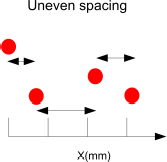
\includegraphics[width = \linewidth]{./pictures/uniform_spacing_1.png}
    	\caption{Con dati grezzi}
    \end{subfigure}
    \hspace{1em}
    \begin{subfigure}{.3\linewidth}
		\centering
		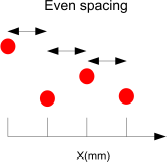
\includegraphics[width = \linewidth]{./pictures/uniform_spacing_2.png}
    	\caption{Con spaziatura uniforme}
    \end{subfigure}
    \caption{Confronto con e senza spaziatura uniforme.}
    \label{fig:uniform_spacing}
\end{figure}

\subsection{Acquisizione intensità}
Con questo metodo, verrà prodotto un valore di intensità (0-255) per ciascun punto scansionato dal laser. In pratica viene misurata la quantità di luce riflessa dall'oggetto.

\subsection{Metodo scelto}
Per i nostri scopi, ovviamente, è stato scelto il metodo dell'acquisizione della superficie con una spaziatura uniforme di 0.15 mm.
\cleardoublepage
\chapter{Analisi}
\label{Cha:analisi}
\thispagestyle{empty}

Il capitolo seguente sarà incentrato sulla presentazione dei prodotti, seguita da una descrizione generale degli algoritmi utilizzati per effettuare le rispettive analisi.

\section{Prodotti}
Per gli esperimenti sono stati usati tre tipi di battistrada diversi. I primi due (figura \ref{fig:batt_1a} e figura \ref{fig:batt_1b})sono molto simili ma differenziano per complessità e numero di blocchi (\textit{blob}), mentre il terzo (figura \ref{fig:batt_2}) è molto differente perchè presenta delle concavità irregolari e delle parti consumate.\\
Da questo momento in poi, per facilitarne la comprensione, ogni battistrada avrà un suo nome specifico.\\

\begin{figure}[H]
	\centering
	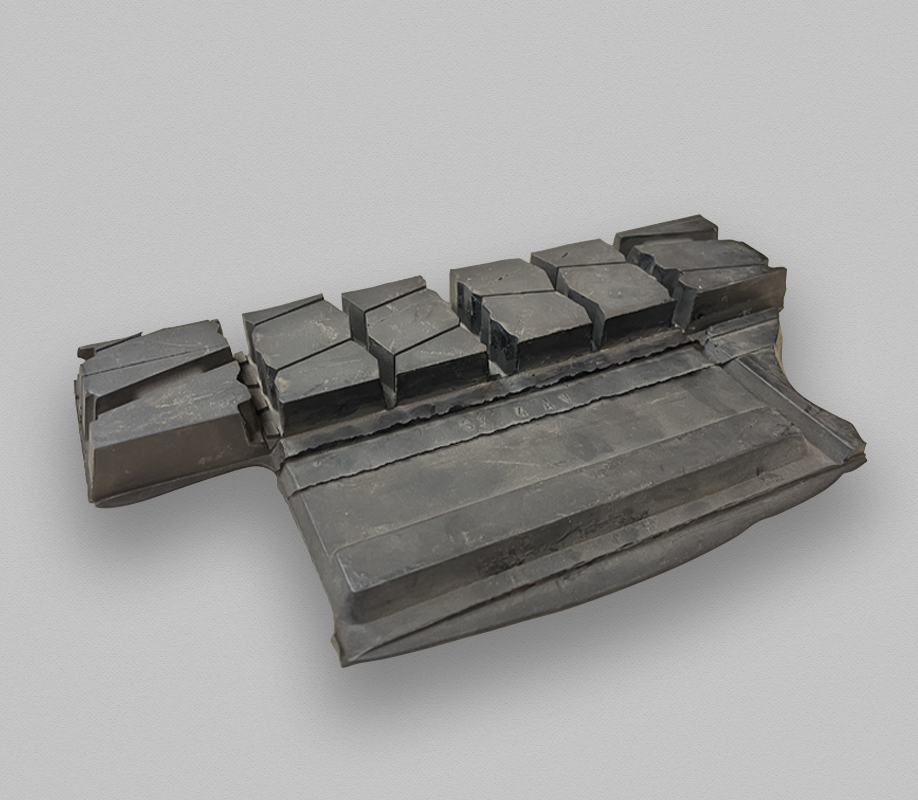
\includegraphics[height=0.41\columnwidth]{./pictures/batt_1a_1.png}
	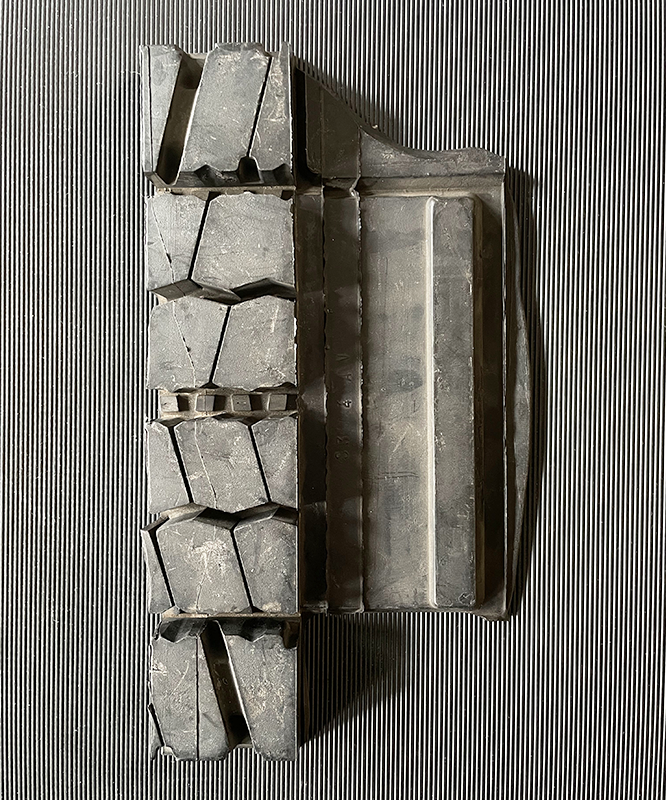
\includegraphics[height=0.41\columnwidth]{./pictures/batt_1a_2.png}
	\caption{Battistrada di tipo \textit{1A}}\label{fig:batt_1a}
\end{figure}

\begin{figure}[H]
	\centering
	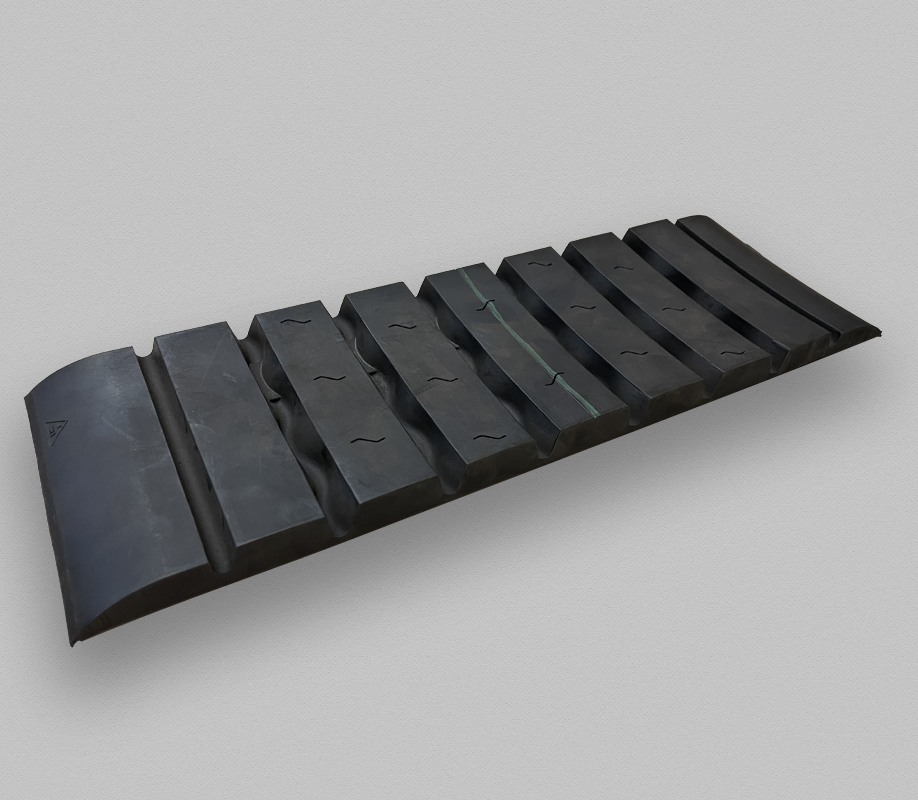
\includegraphics[height=0.41\columnwidth]{./pictures/batt_1b_1.png}
	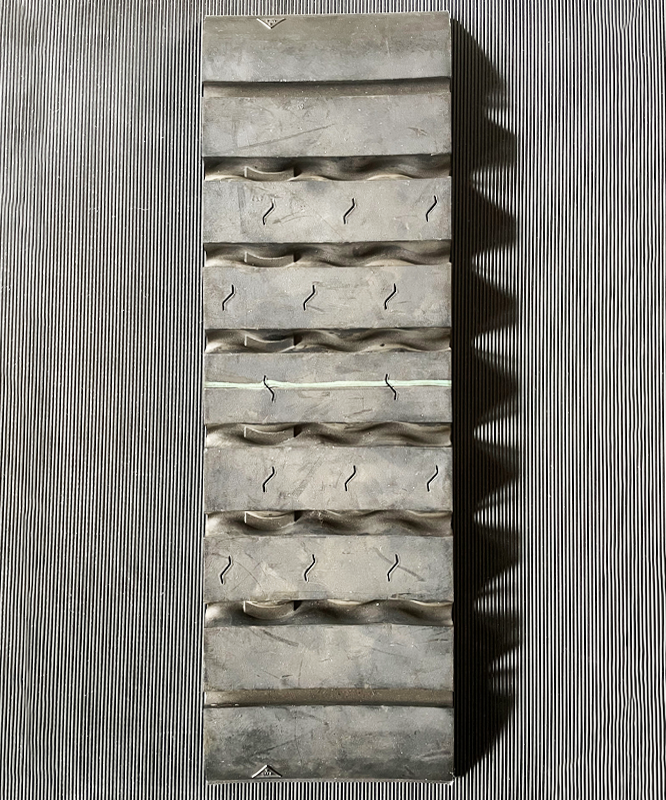
\includegraphics[height=0.41\columnwidth]{./pictures/batt_1b_2.png}
	\caption{Battistrada di tipo \textit{1B}}\label{fig:batt_1b}
\end{figure}

\begin{figure}[H]
	\centering
	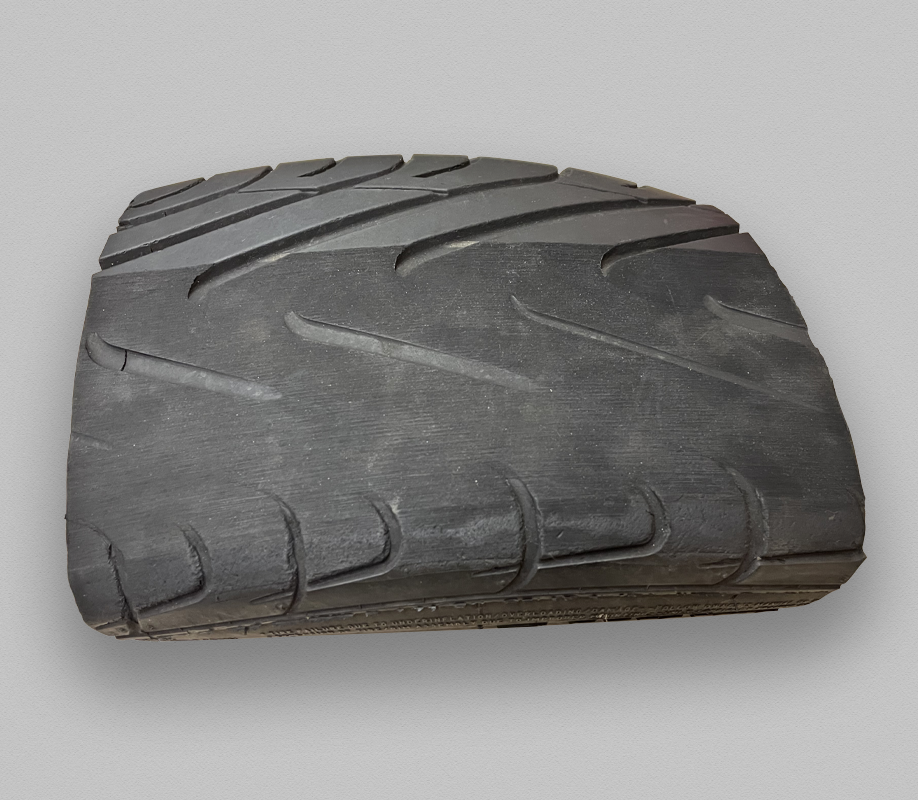
\includegraphics[height=0.41\columnwidth]{./pictures/batt_2_1.png}
	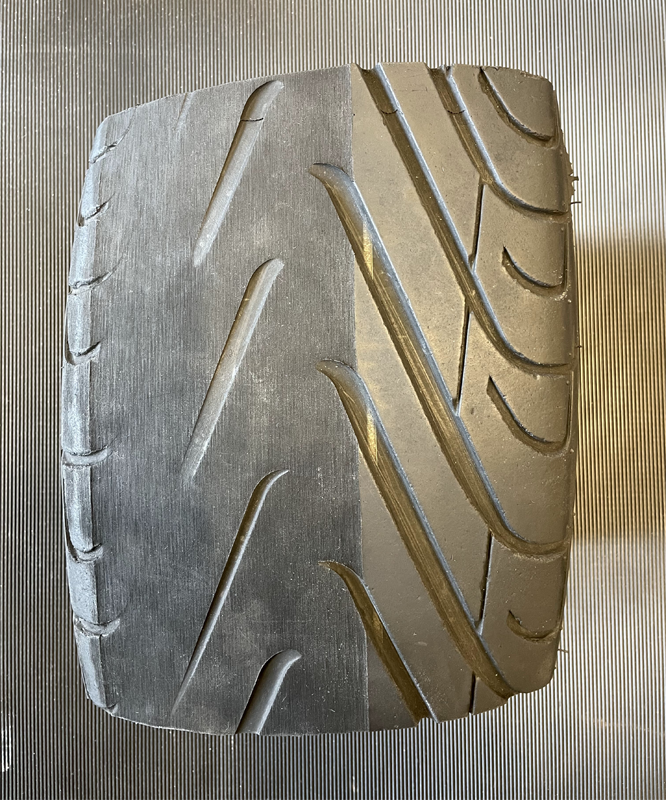
\includegraphics[height=0.41\columnwidth]{./pictures/batt_2_2.png}
	\caption{Battistrada di tipo \textit{2}}\label{fig:batt_2}
\end{figure}

\newpage

\section{Librerie di supporto}
Il programma è stato creato in \textit{C++} e in \textit{C\#}, utilizzando \textit{Visual Studio} come ambiente di sviluppo.\\
\newline
Le librerie utilizzate per realizzare il progetto sono:
\begin{itemize}
	\item \textit{Gocator Software Development Kit (GoSDK), versione 6.1.32.12}, è una libreria open source che può essere utilizzata per accedere e controllare a livello di codice i sensori del Gocator;
	\item \textit{OpenCV, versione 4.5.4}, è una libreria software multipiattaforma nell'ambito della visione artificiale in tempo reale;
	\item \textit{Point Cloud Library, versione 1.12.1}, è una libreria open source di algoritmi per le attività di elaborazione delle nuvole di punti e l'elaborazione della geometria 3D;
	\item \textit{GNU Scientific Library, versione 2.7}, è una libreria di software per calcoli numerici in matematica e scienze applicate;
	\item \textit{JSON for Modern C++, versione 3.10.5}, è una libreria per elaborare dati in formato \textit{JSON};
	\item \textit{Helix Toolkit, versione 2.20.2}, è una raccolta di componenti 3D per \textit{.NET};
	\item \textit{Json.NET - Newtonsoft, versione 13.0.1}, è un popolare framework JSON ad alte prestazioni per \textit{.NET};
	\item \textit{Ookii.Dialogs.Wpf, versione 5.0.1}, è una libreria per applicazioni \textit{WPF}.
\end{itemize}

\section{Algoritmi di analisi}

\subsection{Battistrada di tipo 1A/1B}
Dall'analisi di questo tipo di battistrada si è deciso di estrarre le seguenti features:
\begin{itemize}
	\item Distanza minima tra ogni \textit{MacroBlob} adiacente \textbf{(1A/1B)}.
	\item Area, perimetro e dimensione della \textit{bounding box} di ogni \textit{MacroBlob} \textbf{(1A/1B)}.
	\item Area, perimetro e dimensione della \textit{bounding box} di ogni \textit{Blob} \textbf{(1A)}.
	\item Per ogni \textit{MacroBlob}, la distanza minima tra ogni \textit{Blob} adiacente \textbf{(1A)}.
\end{itemize}

\noindent Successivamente, per fini statistici, si è calcolato il minimo, il massimo e la media dei valori trovati in elenco.\\
\newline
Prendendo come esempio il battistrada di tipo \textit{1A}, nella figura \ref{fig:batt_1a_analisi_mb} sono evidenziati i \textit{MacroBlob}, mentre nella figura \ref{fig:batt_1a_analisi_b} i \textit{Blob}.\\
Nel caso del battistrada di tipo \textit{1B} (figura \ref{fig:batt_1b_analisi_mb}), parliamo solo di \textit{MacroBlob} perchè non sono presenti blocchi interni.\\

\begin{figure}[H]
	\centering
	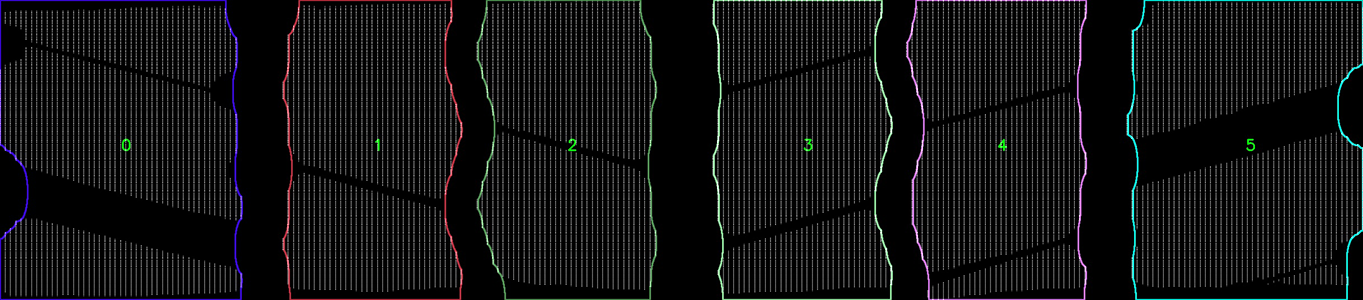
\includegraphics[width=0.9\columnwidth]{./pictures/batt_1a_analisi_mb.png}
	\caption{Contorni dei MacroBlob, in questo ne sono presenti 6.}\label{fig:batt_1a_analisi_mb}
\end{figure}

\begin{figure}[H]
	\centering
	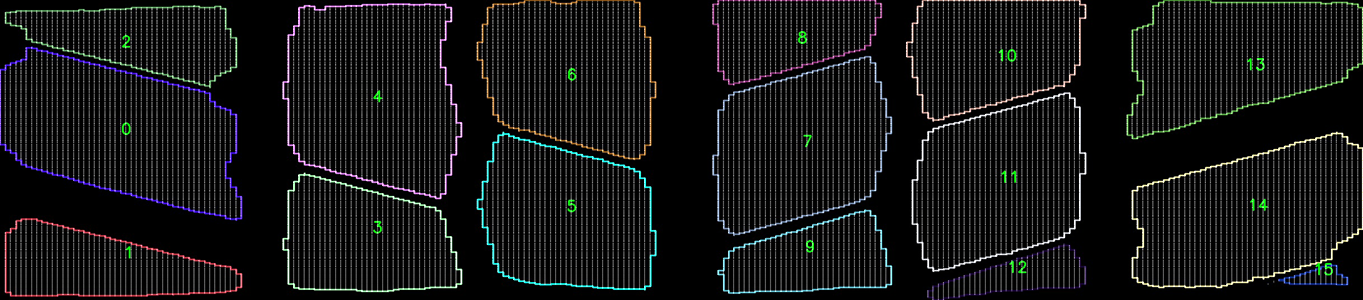
\includegraphics[width=0.9\columnwidth]{./pictures/batt_1a_analisi_b.png}
	\caption{Contorni dei Blob, in questo caso ne sono presenti 16.}\label{fig:batt_1a_analisi_b}
\end{figure}

\begin{figure}[H]
	\centering
	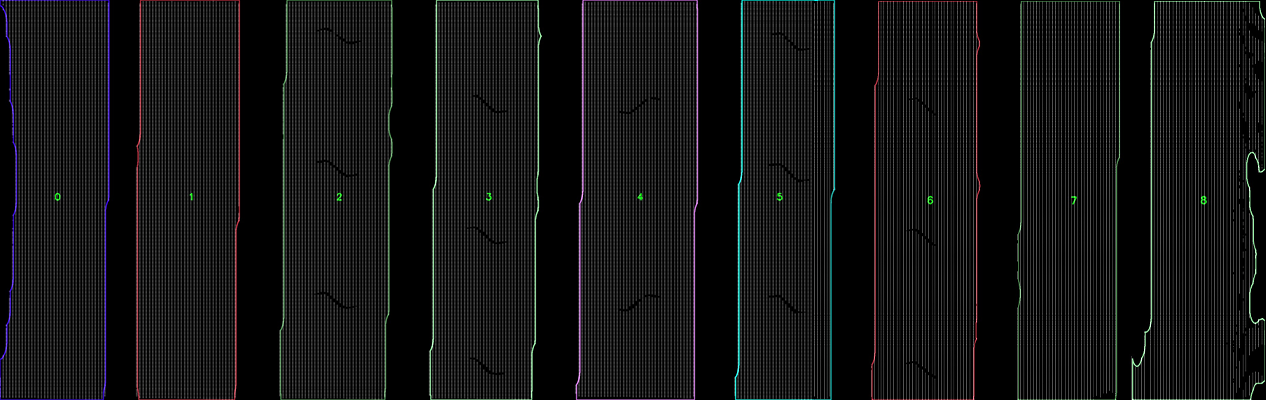
\includegraphics[width=0.9\columnwidth]{./pictures/batt_1b_analisi_mb.png}
	\caption{Contorni dei MacroBlob, in questo caso ne sono presenti 9.}\label{fig:batt_1b_analisi_mb}
\end{figure}

\noindent In seguito alla scansione dell'oggetto, da parte del profilometro laser, ciò che abbiamo non sono altro che delle coordinate \textit{x}, \textit{y} e \textit{z} dove sono definiti tutti i punti presenti nella \textit{point cloud}, dove il punto (0,0,0) coincide con il centro del piano della stessa (figura \ref{fig:batt_1a_analisi_1}).\\

\begin{figure}[H]
	\centering
	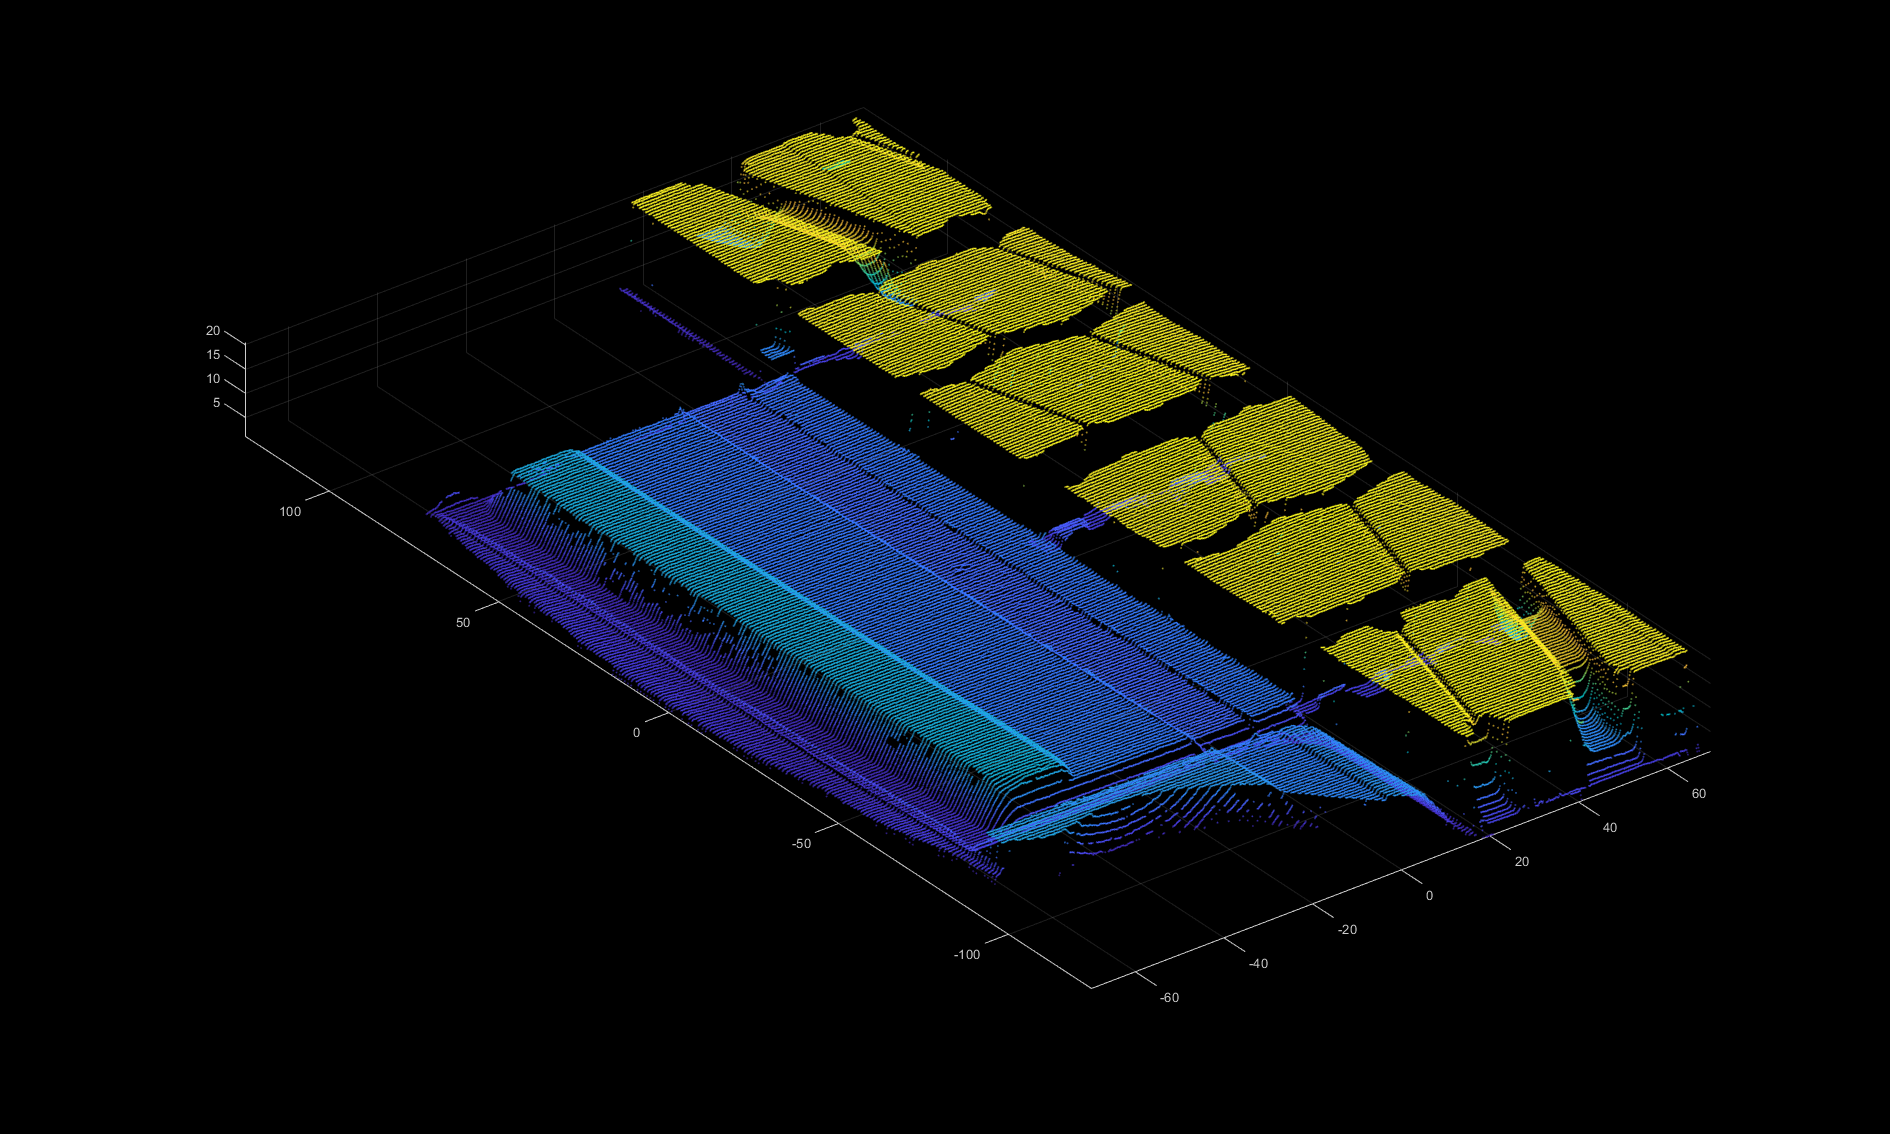
\includegraphics[width=0.8\columnwidth]{./pictures/batt_1a_analisi_1.png}
	\caption{Point cloud non elaborata del battistrada di tipo \textit{1A}.}\label{fig:batt_1a_analisi_1}
\end{figure}

\noindent La prima operazione effettuata è stata quella di applicare un filtro per rimuovere eventuali misurazioni rumorose, come ad esempio valori anomali. Infatti, le scansioni laser, generando \textit{point cloud} con una densità di punti variabile, effettuano spesso errori di misurazione che riportano valori anomali.\\
\newline
Per evitare il più possibile questi errori, è stata applicata un'analisi statistica sull'intorno di ciascun punto, filtrando quelli che non soddisfano un determinato criterio. Assumendo che la distribuzione risultante sia gaussiana con una media e una deviazione standard, tutti i punti le cui distanze medie sono al di fuori di un intervallo definito dalla media delle distanze globali e dalla deviazione standard, possono essere considerati valori anomali e quindi rimossi.\\
\newline
La figura \ref{fig:batt_1a_analisi_2} mostra gli effetti dell'analisi e della rimozione dei valori anomali.

\begin{figure}[H]
	\centering
	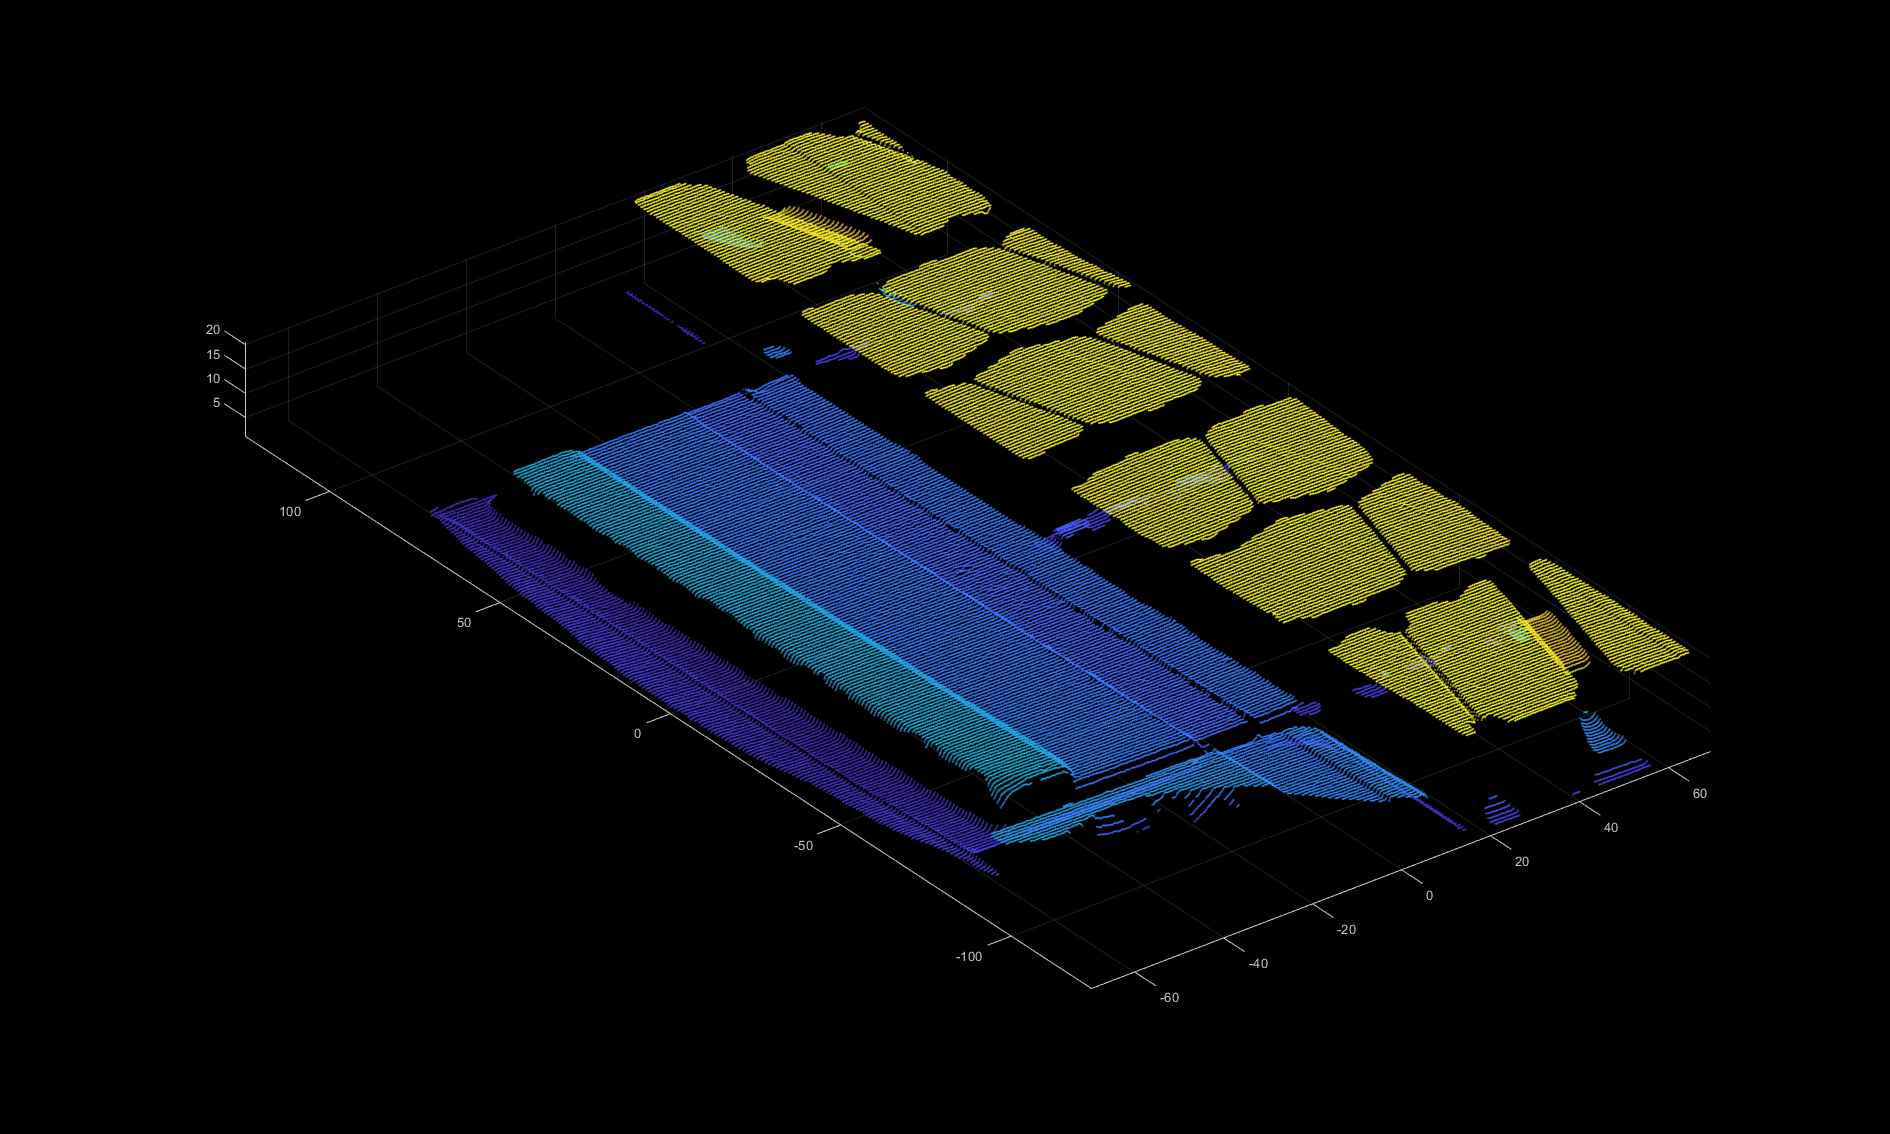
\includegraphics[width=0.8\columnwidth]{./pictures/batt_1a_analisi_2.png}
	\caption{Point cloud del battistrada di tipo \textit{1A} dopo aver applicato il filtro statistico.}\label{fig:batt_1a_analisi_2}
\end{figure}

\noindent Il nuovo obiettivo è quello di mascherare solo la parte dove si trovano i \textit{Blob} (punti di colore giallo della figura \ref{fig:batt_1a_analisi_2}). Per fare ciò, è stata eseguita una semplice segmentazione piana di un insieme di punti, ovvero sono stati trovati tutti i punti all'interno della nostra \textit{point cloud} che supportano un modello piano.\\
\newline
Dopo aver impostato il modello (\textit{pcl::SACMODEL\_PLANE}) e il tipo di metodo (\textit{pcl::SAC\_RANSAC}), è stata specificata una distanza di soglia che determina quanto un punto deve essere vicino al modello piano per essere considerato facente parte del modello stesso.\\
\newline
In questo caso è stata effettuata una prima distinzione tra il battistrada di tipo \textit{1A} e quello di tipo \textit{1B}, perchè sono state impostate diverse distanze di soglia per ognuno.

\begin{figure}[H]
	\centering
	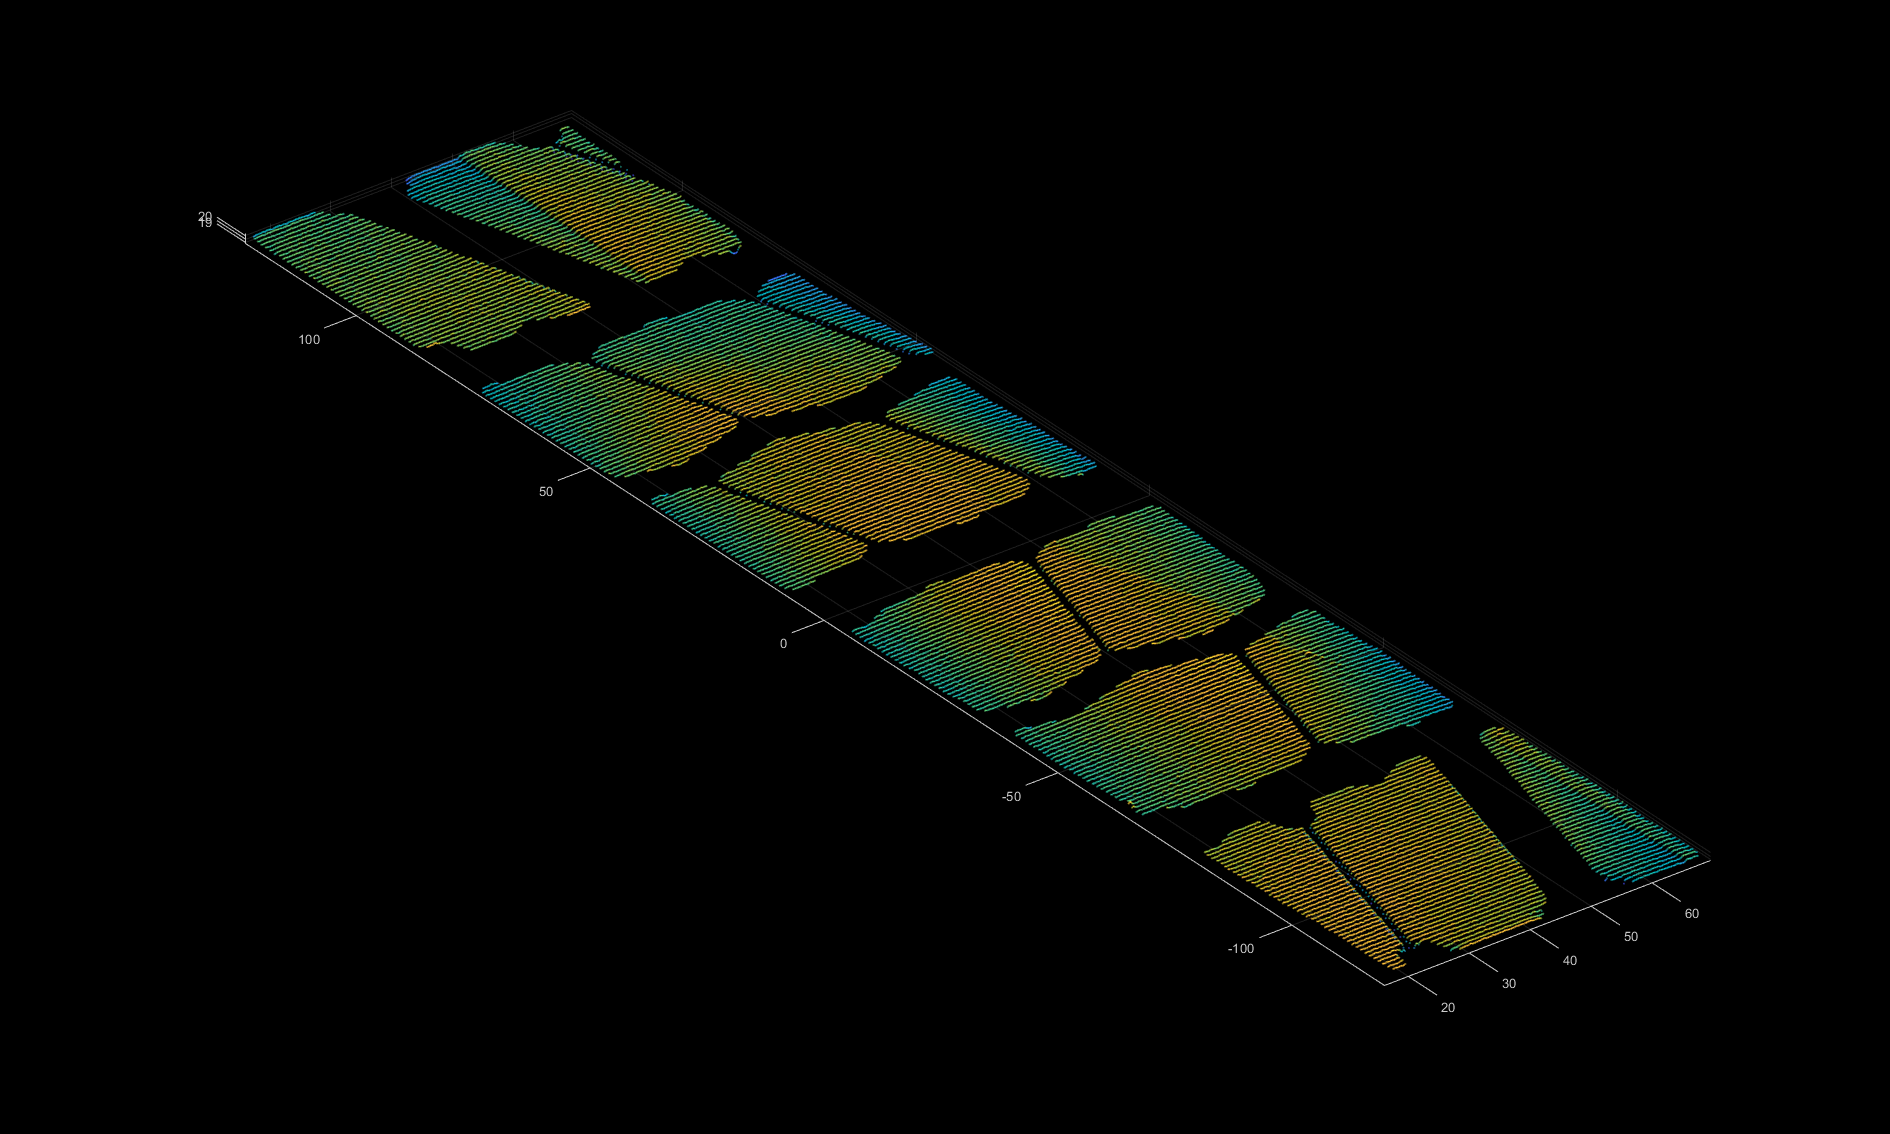
\includegraphics[width=0.8\columnwidth]{./pictures/batt_1a_analisi_3.png}
	\caption{Point cloud del battistrada di tipo \textit{1A} dopo aver applicato la segmentazione planare.}\label{fig:batt_1a_analisi_3}
\end{figure}

\noindent Le ultime due operazioni sulla \textit{point cloud} sono le più semplici. Prima, tutti i punti sono stati proiettati sul piano dato dalla sua equazione \textit{z = 0} (figura \ref{fig:batt_1a_analisi_4}), poi è stata effettuata un operazione di traslazione di tutti i punti portando l'origine degli assi nella posizione convenzionale di un immagine, in alto a sinistra (figura \ref{fig:batt_1a_analisi_5}).\\

\begin{figure}[H]
	\centering
	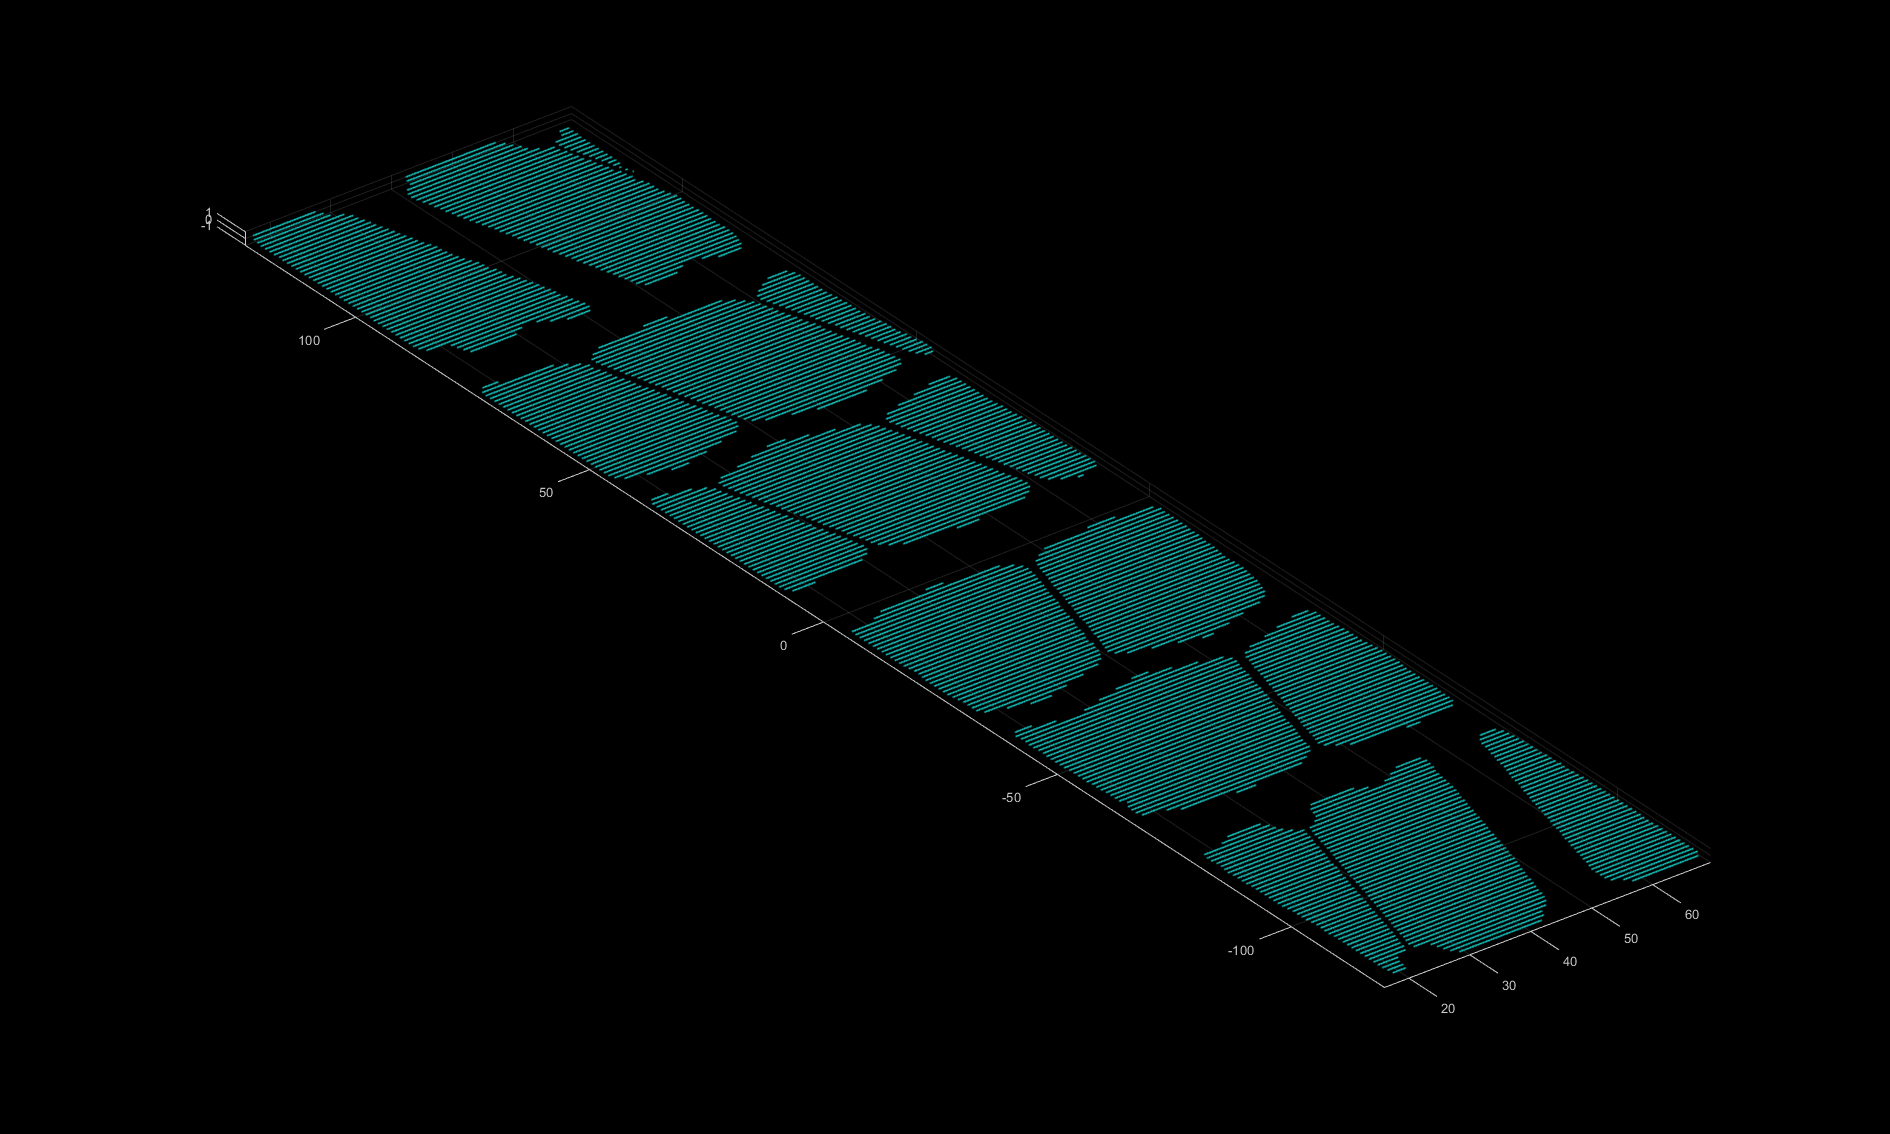
\includegraphics[width=0.8\columnwidth]{./pictures/batt_1a_analisi_4.png}
	\caption{Point cloud del battistrada di tipo \textit{1A} dopo aver applicato l'operazione di proiezione.}\label{fig:batt_1a_analisi_4}
\end{figure}

\begin{figure}[H]
	\centering
	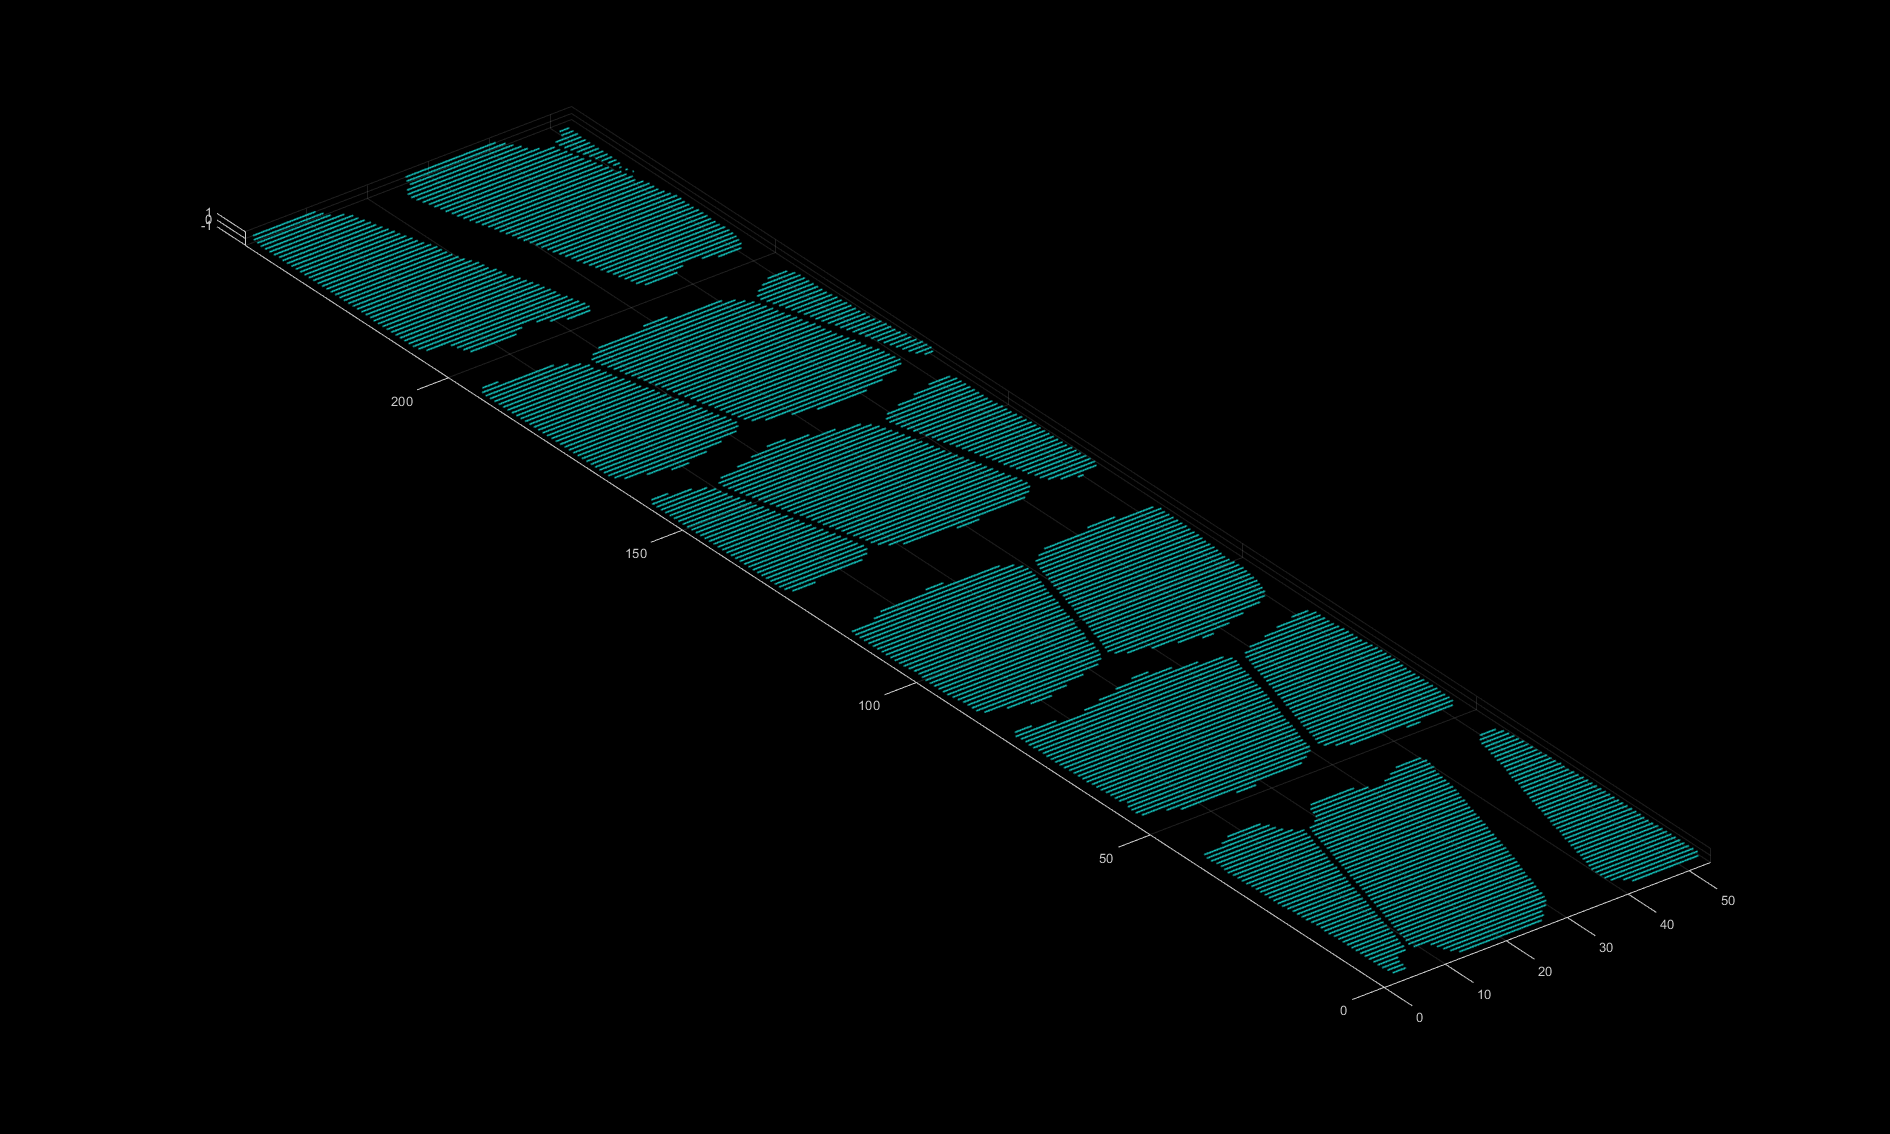
\includegraphics[width=0.8\columnwidth]{./pictures/batt_1a_analisi_5.png}
	\caption{Point cloud del battistrada di tipo \textit{1A} dopo aver applicato l'operazione di traslazione.}\label{fig:batt_1a_analisi_5}
\end{figure}

\noindent A questo punto, per trovare i contorni e le misure dei vari blocchi, si è deciso di utilizzare la libreria \textit{opencv} e quindi è stato necessario creare un immagine dove i punti della \textit{point cloud} sono stati colorati di bianco e tutto il resto di nero.\\
Inoltre è stato applicato un moltiplicatore x10 cosicché 1 pixel dell'immagine corrispondesse, nel mondo reale, ad 1 µm.\\

\begin{figure}[H]
	\centering
	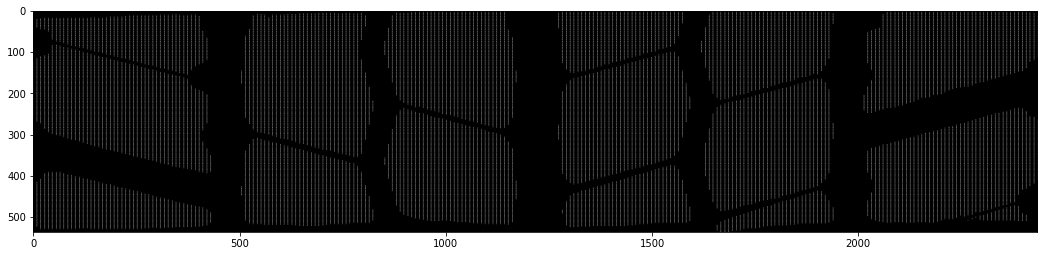
\includegraphics[width=0.9\columnwidth]{./pictures/batt_1a_analisi_6.png}
	\caption{Immagine planare del battistrada di tipo \textit{1A}.}\label{fig:batt_1a_analisi_6}
\end{figure}

\noindent Per chiudere i piccoli fori presenti nei \textit{Blob} della figura \ref{fig:batt_1a_analisi_6}, sono state usate delle trasformazioni morfologiche, in particolare di tipo \textit{closing}.\\
\newline
Le trasformazioni morfologiche sono delle operazioni che si basano sulla forma dell'immagine. L'operazione di tipo \textit{closing} non è altro che il susseguirsi di due operatori: prima viene applicata una \textit{dilatazione} e poi un \textit{erosione}.\\
La figura \ref{fig:batt_1a_analisi_7} è il risultato della prima \textit{closing} applicata per trovare i \textit{Blob}, mentre la figura \ref{fig:batt_1a_analisi_8} è il risultato della \textit{closing} applicata all'immagine precedente per trovare i \textit{MacroBlob}.\\

\begin{figure}[H]
	\centering
	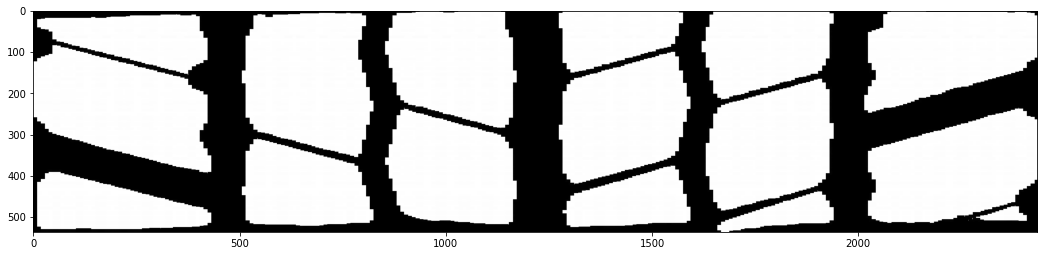
\includegraphics[width=0.9\columnwidth]{./pictures/batt_1a_analisi_7.png}
	\caption{Immagine del battistrada di tipo \textit{1A} dopo aver applicato la prima trasformazione morfologica (Closing).}\label{fig:batt_1a_analisi_7}
\end{figure}

\begin{figure}[H]
	\centering
	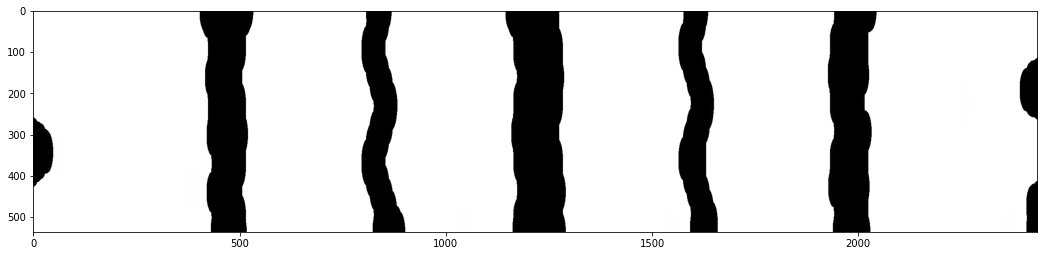
\includegraphics[width=0.9\columnwidth]{./pictures/batt_1a_analisi_8.png}
	\caption{Immagine del battistrada di tipo \textit{1A} dopo aver applicato la seconda trasformazione morfologica (Closing).}\label{fig:batt_1a_analisi_8}
\end{figure}

\noindent Quindi per trovare i contorni è stata utilizzata la funzione \textit{findContours()} di \textit{opencv} che accetta come argomenti: l'immagine sorgente in scala di grigio, la modalità di recupero (\textit{cv::RETR\_EXTERNAL}) e il metodo di approssimazione (\textit{cv::CHAIN\_APPROX\_NONE}) del contorno.\\
\newline
Una volta trovate tutte le coordinate dei punti dei contorni, è risultato immediato calcolare area (\textit{cv::contourArea()}) e perimetro (\textit{cv::arcLength()}). Per quanto riguarda le altre misure, si è preferito ricavarle dalle \textit{bounding box} di ogni blocco come si può vedere nelle figure \ref{fig:batt_1a_analisi_10} e \ref{fig:batt_1a_analisi_12}.\\
\newline
Per distinguere il battistrada di tipo \textit{1A} da quello di tipo \textit{1B}, è stata inserita, nel codice, la condizione che se il numero di \textit{Blob} e \textit{MacroBlob} trovati fosse uguale allora non si prosegue nel trovare la distanza minima tra \textit{Blob} in quanto sarebbe uguale a quella tra \textit{MacroBlob}.

\begin{figure}[H]
	\centering
	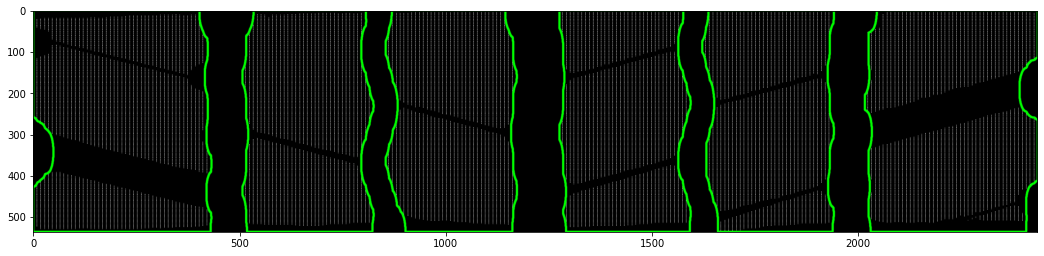
\includegraphics[width=0.9\columnwidth]{./pictures/batt_1a_analisi_9.png}
	\caption{Immagine del battistrada di tipo \textit{1A} con i contorni dei MacroBlob evidenziati.}\label{fig:batt_1a_analisi_9}
\end{figure}

\begin{figure}[H]
	\centering
	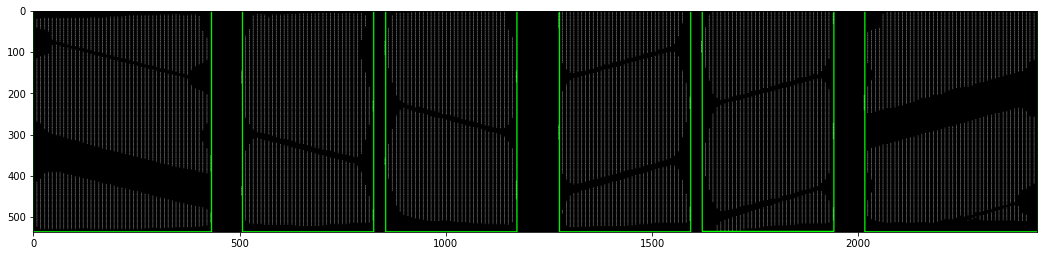
\includegraphics[width=0.9\columnwidth]{./pictures/batt_1a_analisi_10.png}
	\caption{Immagine del battistrada di tipo \textit{1A} con le bounding box dei MacroBlob evidenziate.}\label{fig:batt_1a_analisi_10}
\end{figure}

\begin{figure}[H]
	\centering
	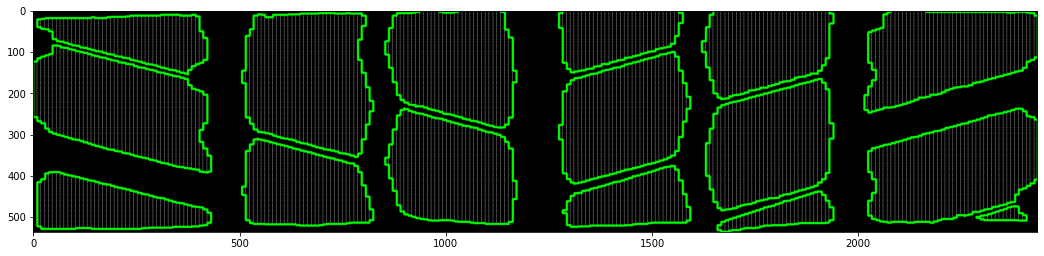
\includegraphics[width=0.9\columnwidth]{./pictures/batt_1a_analisi_11.png}
	\caption{Immagine del battistrada di tipo \textit{1A} con i contorni dei Blob evidenziati.}\label{fig:batt_1a_analisi_11}
\end{figure}

\begin{figure}[H]
	\centering
	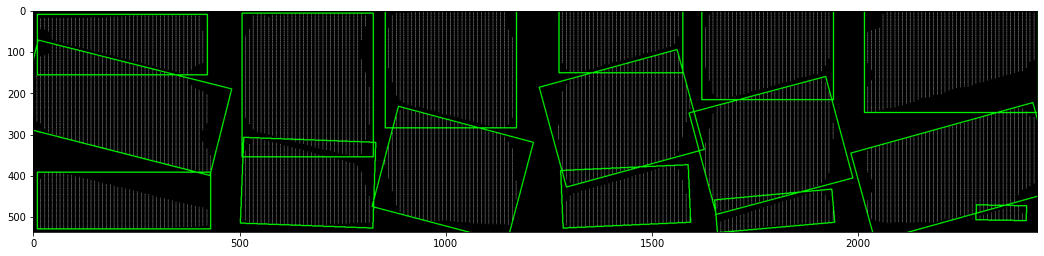
\includegraphics[width=0.9\columnwidth]{./pictures/batt_1a_analisi_12.png}
	\caption{Immagine del battistrada di tipo \textit{1A} con le bounding box dei Blob evidenziate.}\label{fig:batt_1a_analisi_12}
\end{figure}

\noindent Per trovare la distanza minima tra \textit{Blob} adiacenti presenti in ogni \textit{MacroBlob} è stata creata una funzione specifica che confronta le varie distanze tra i centri dei \textit{Blob}.

% \cppexternal{./codes/f.cpp}

\noindent Di seguito vengono illustrati i passaggi seguiti per il battistrada di tipo \textit{1B}.\\

\begin{figure}[H]
	\centering
	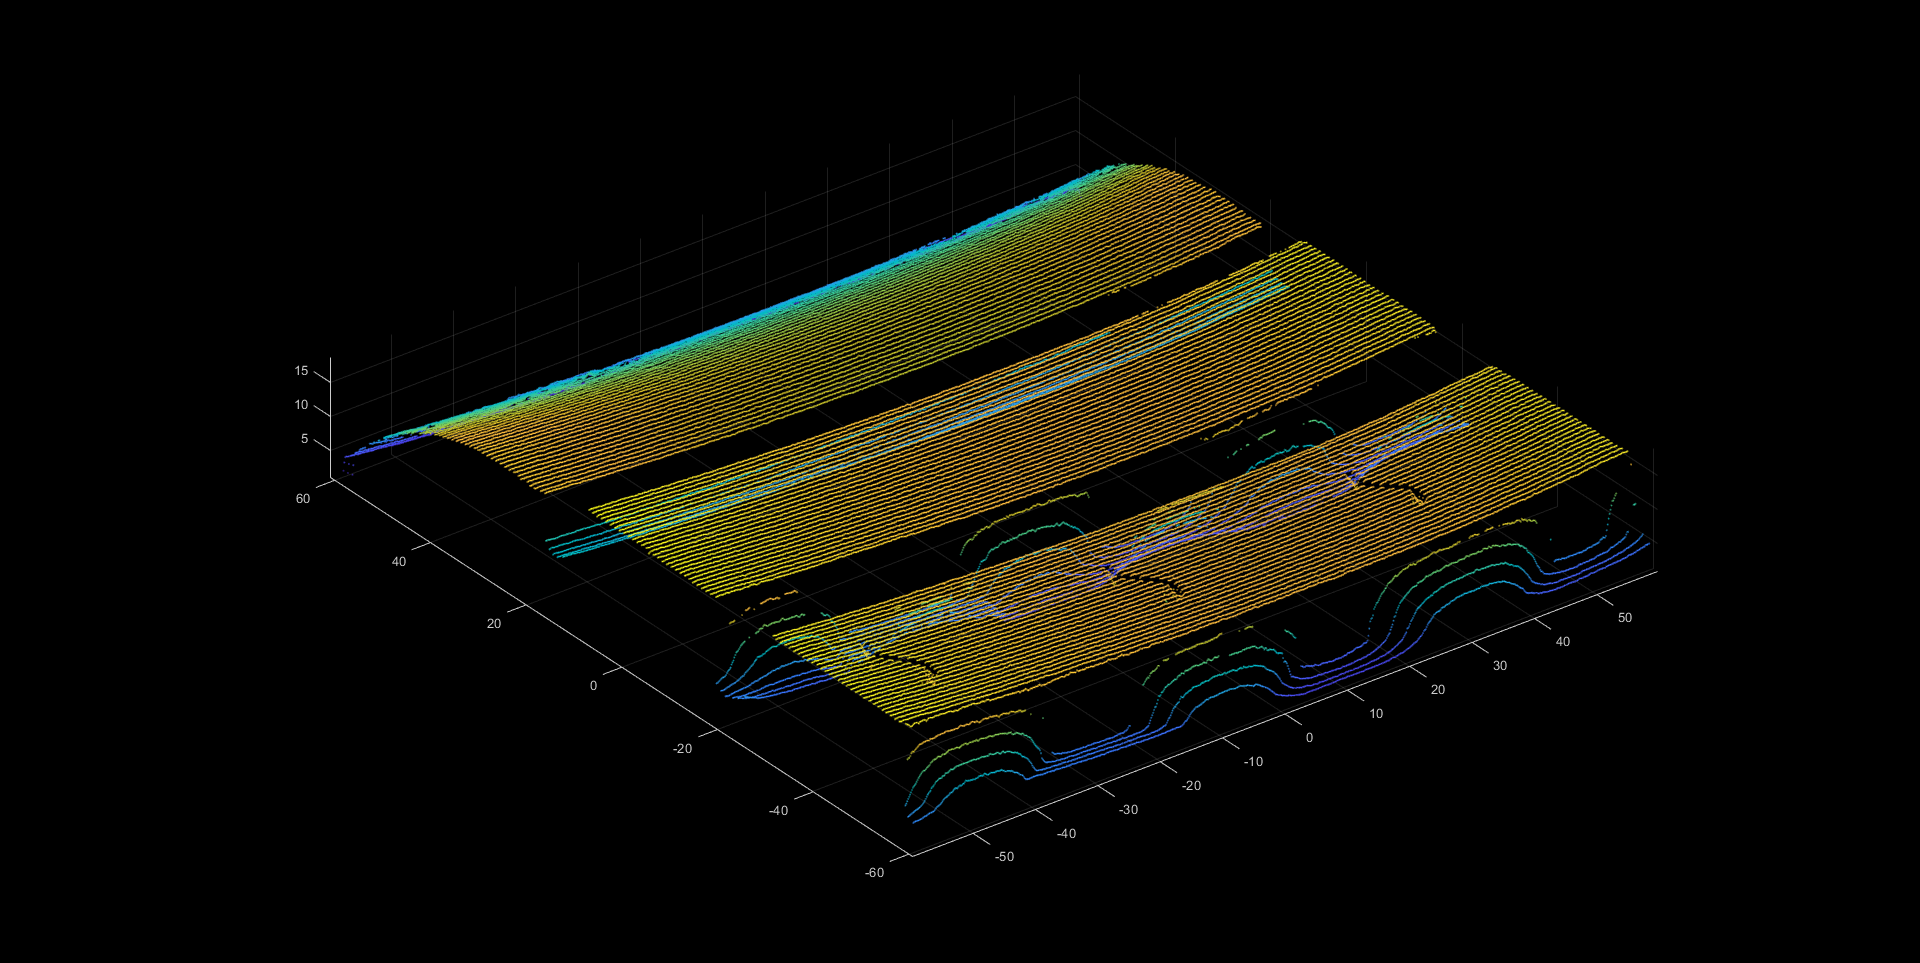
\includegraphics[width=0.45\columnwidth]{./pictures/batt_1b_analisi_1_1.png}
	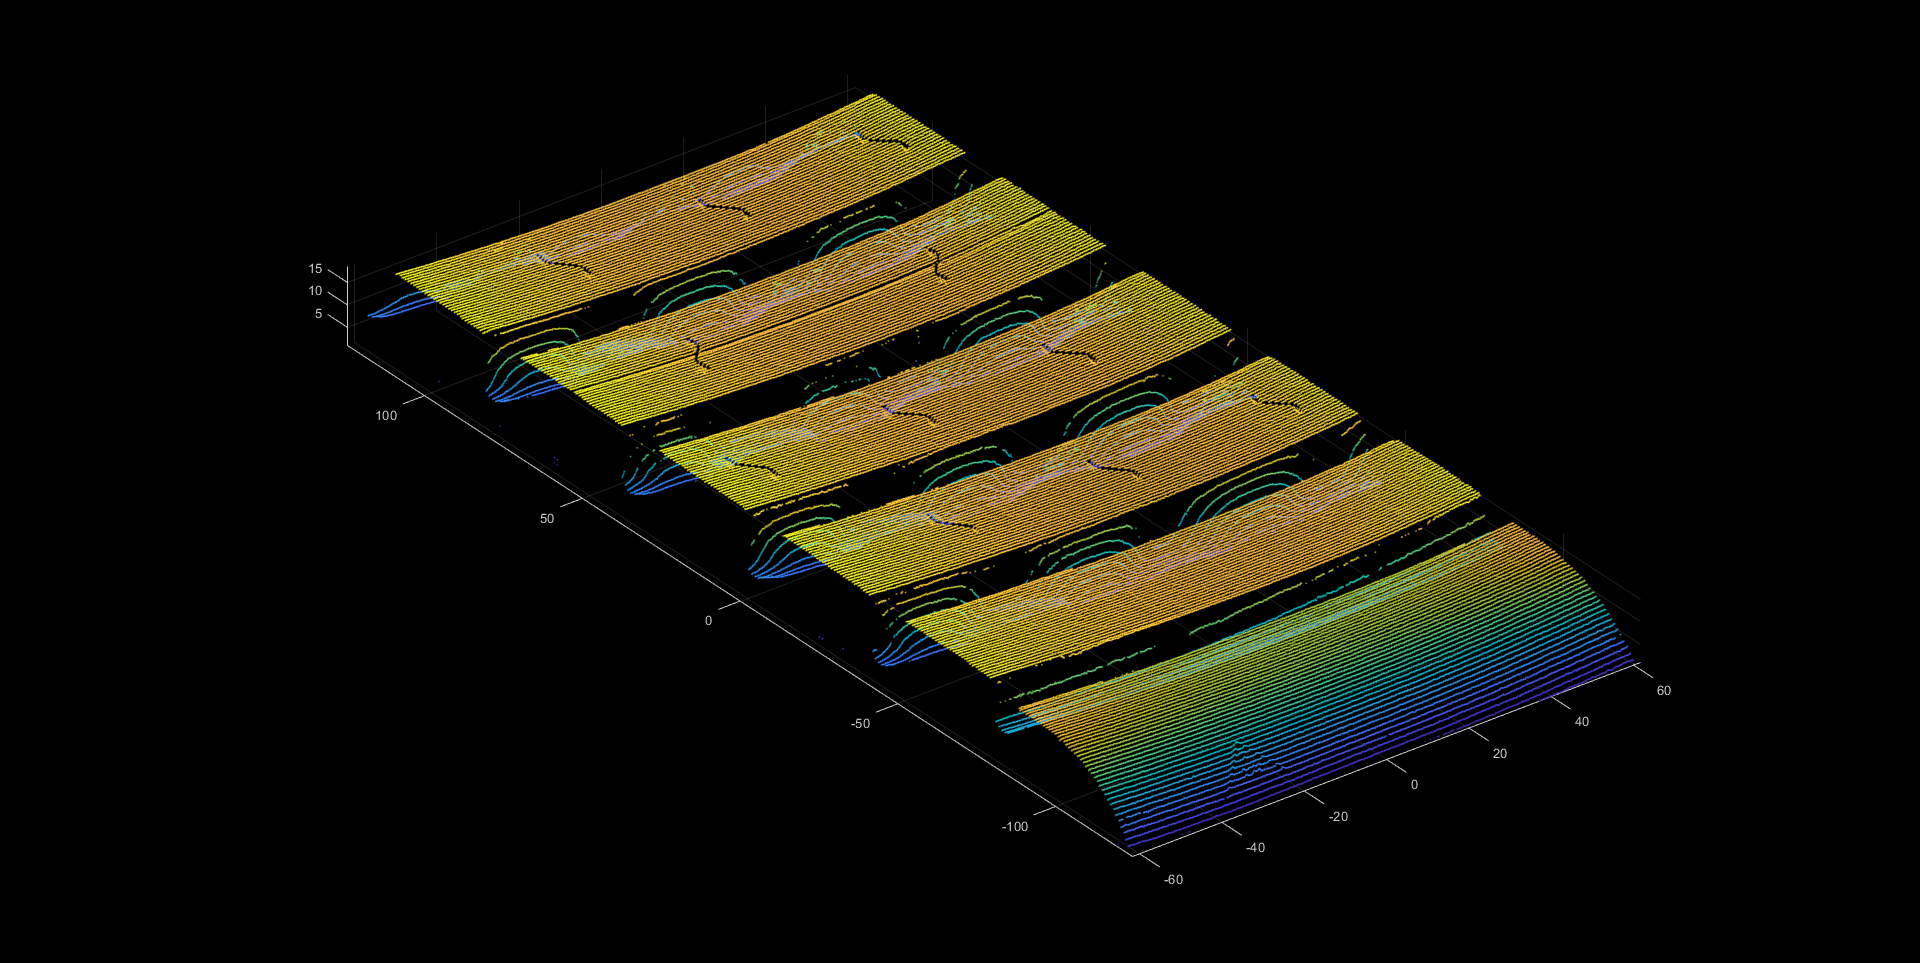
\includegraphics[width=0.45\columnwidth]{./pictures/batt_1b_analisi_2_1.png}
	\caption{Point cloud non elaborata del battistrada di tipo \textit{1B}.}\label{fig:batt_1b_analisi_1}
\end{figure}

\begin{figure}[H]
	\centering
	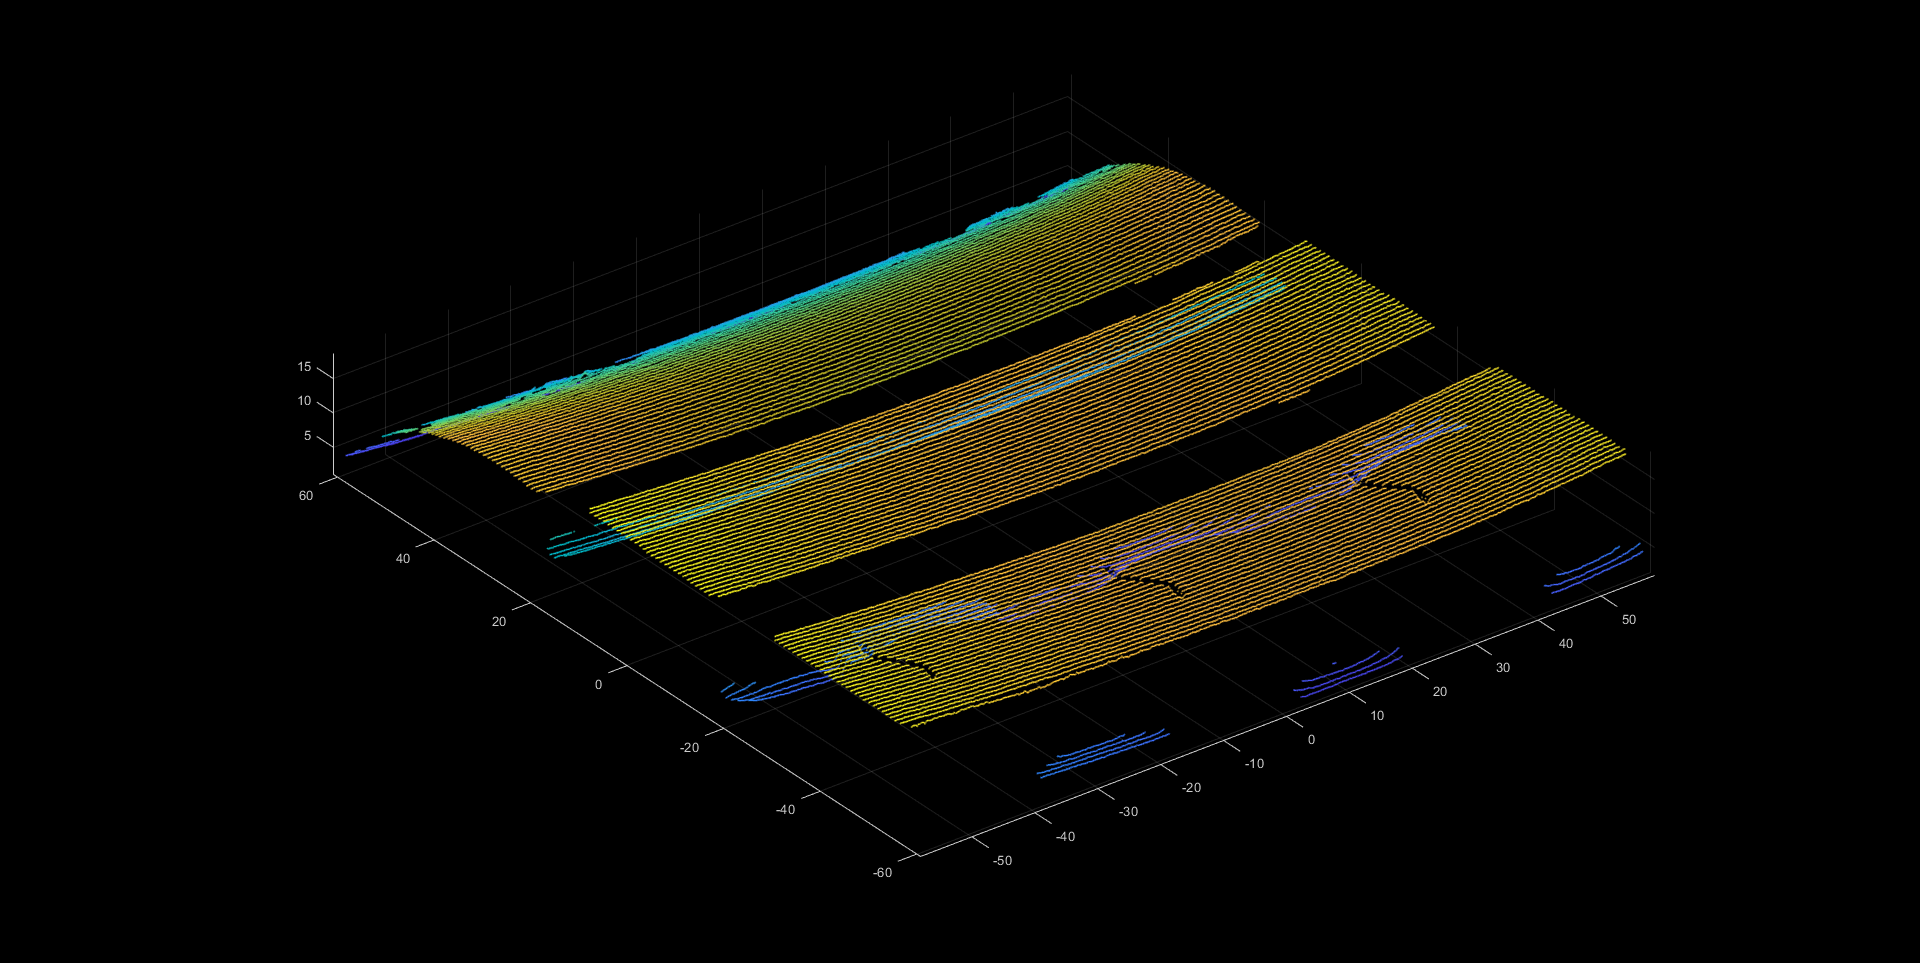
\includegraphics[width=0.45\columnwidth]{./pictures/batt_1b_analisi_1_2.png}
	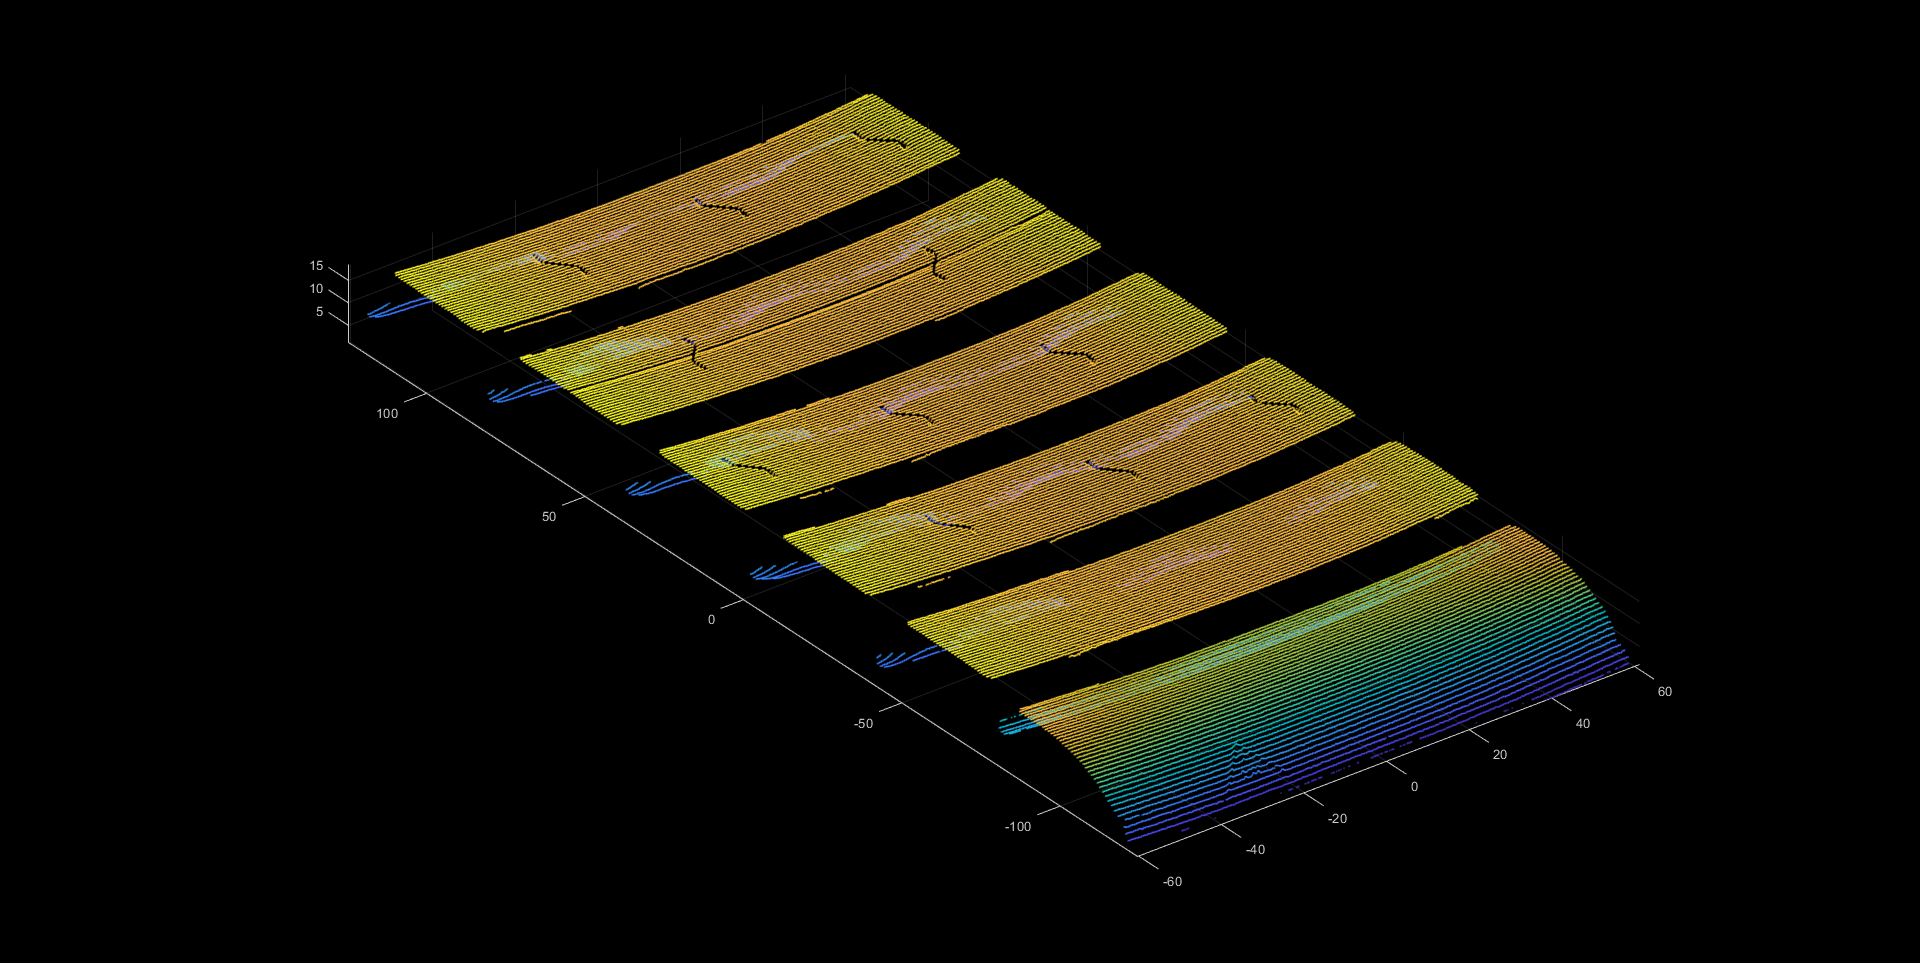
\includegraphics[width=0.45\columnwidth]{./pictures/batt_1b_analisi_2_2.png}
	\caption{Point cloud del battistrada di tipo \textit{1B} dopo aver applicato il filtro statistico.}\label{fig:batt_1b_analisi_2}
\end{figure}

\begin{figure}[H]
	\centering
	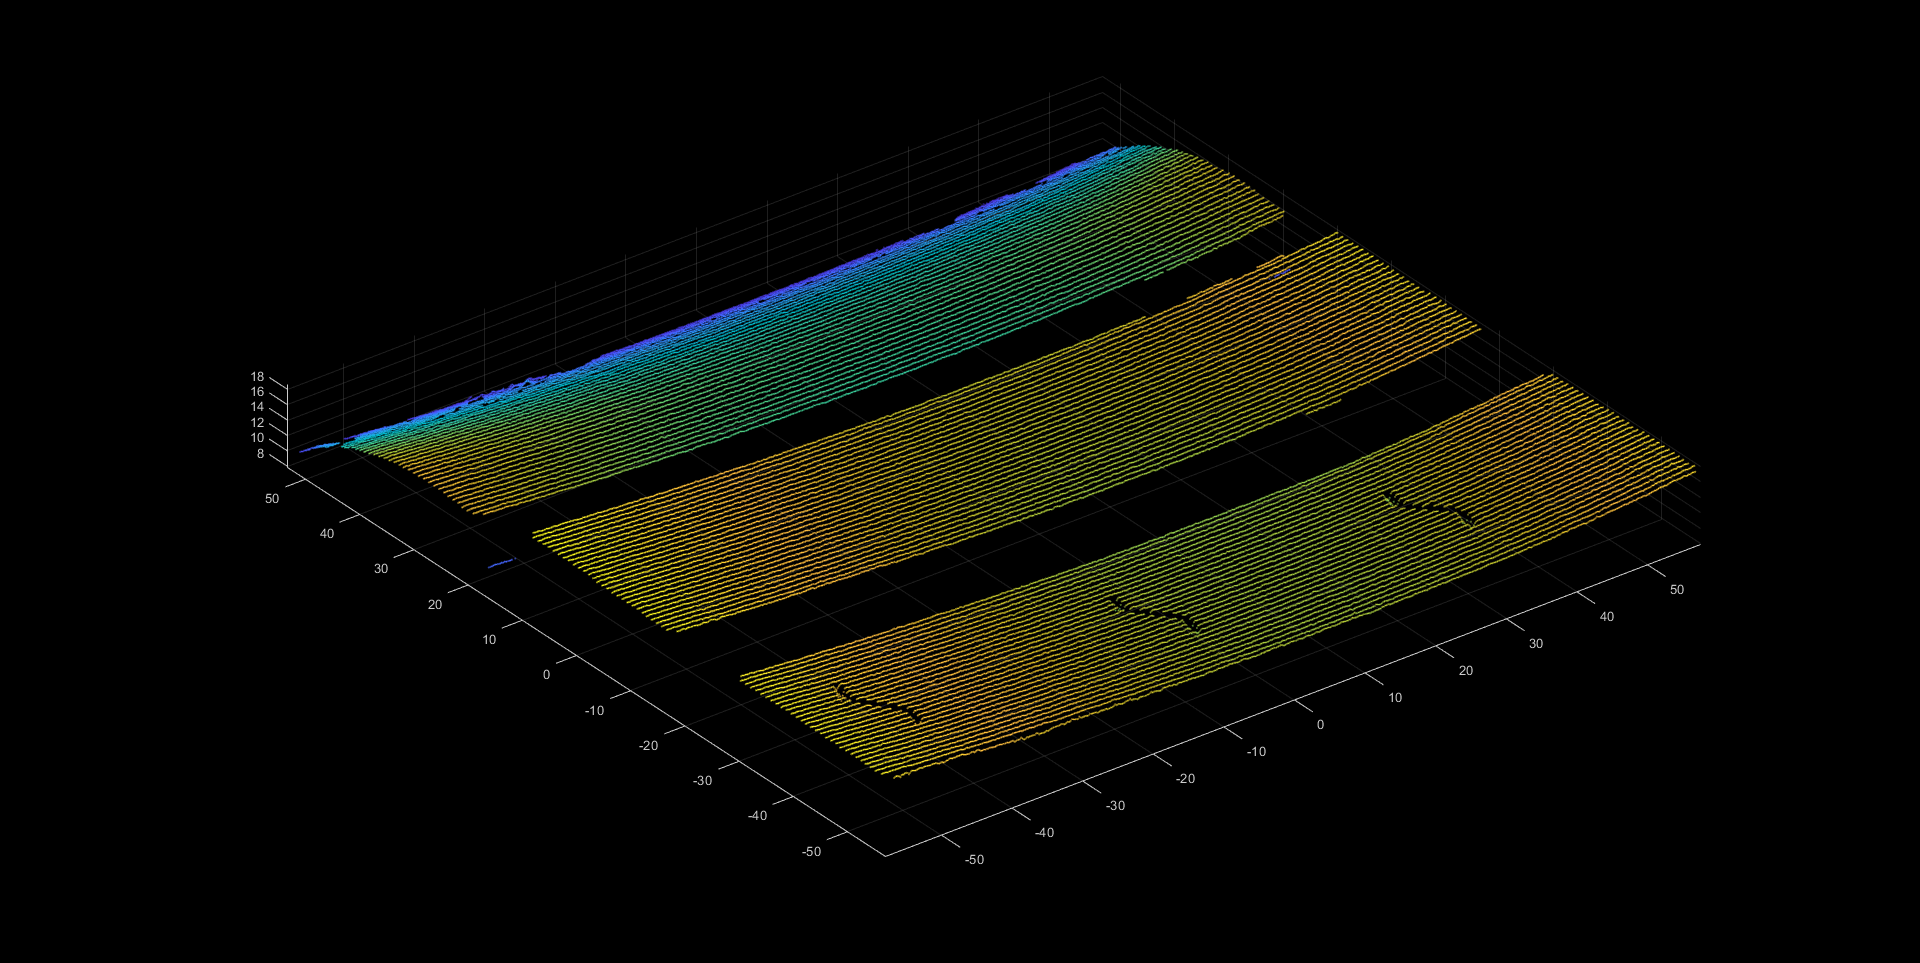
\includegraphics[width=0.45\columnwidth]{./pictures/batt_1b_analisi_1_3.png}
	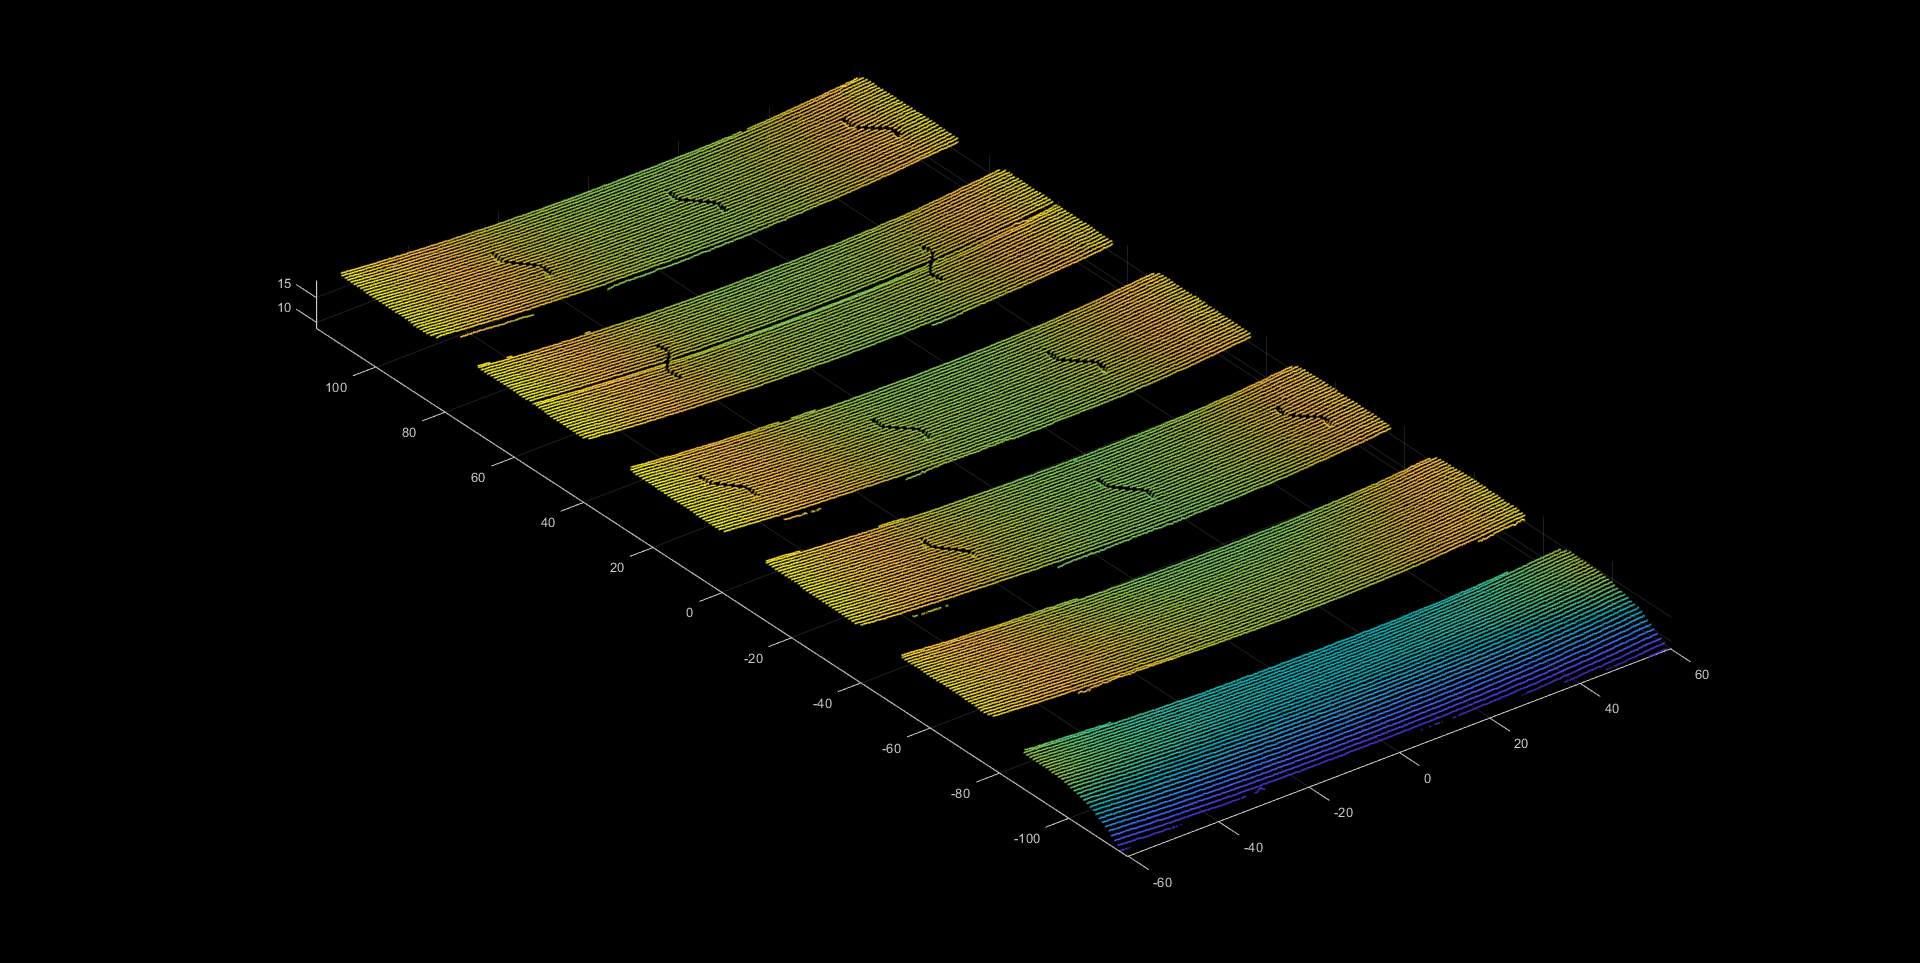
\includegraphics[width=0.45\columnwidth]{./pictures/batt_1b_analisi_2_3.png}
	\caption{Point cloud del battistrada di tipo \textit{1B} dopo aver applicato la segmentazione planare.}\label{fig:batt_1b_analisi_3}
\end{figure}

\begin{figure}[H]
	\centering
	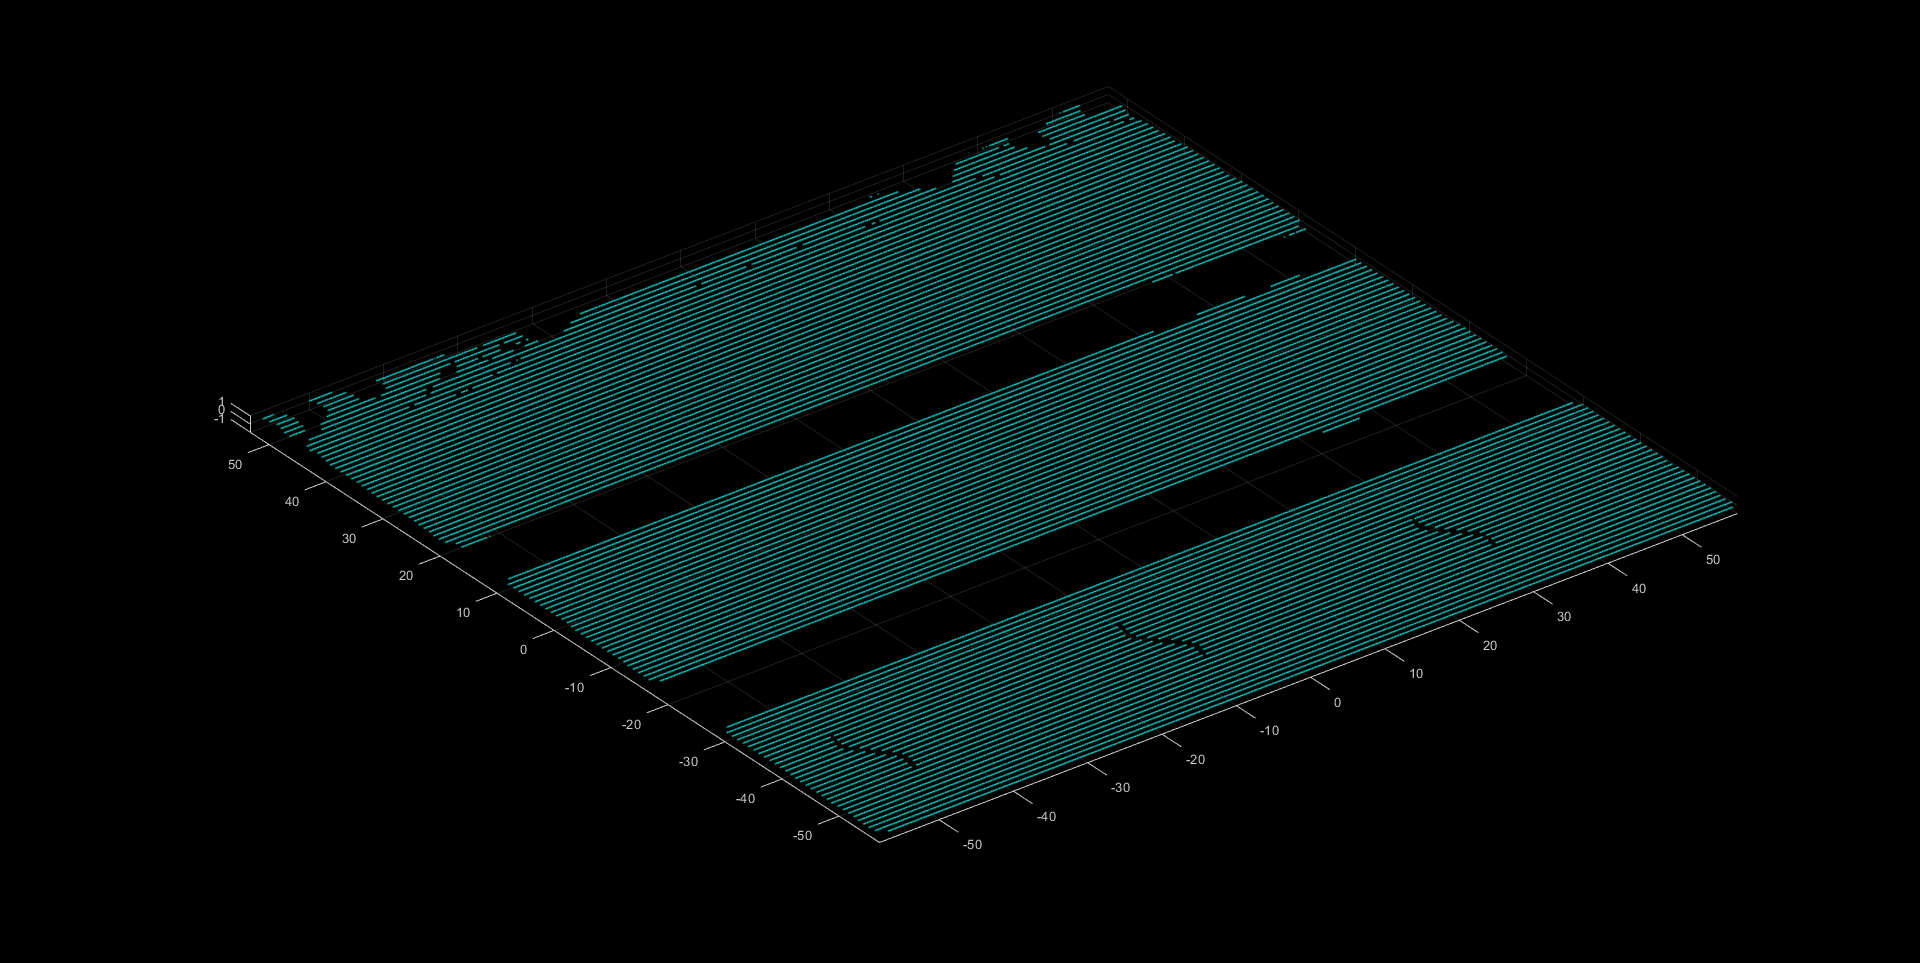
\includegraphics[width=0.45\columnwidth]{./pictures/batt_1b_analisi_1_4.png}
	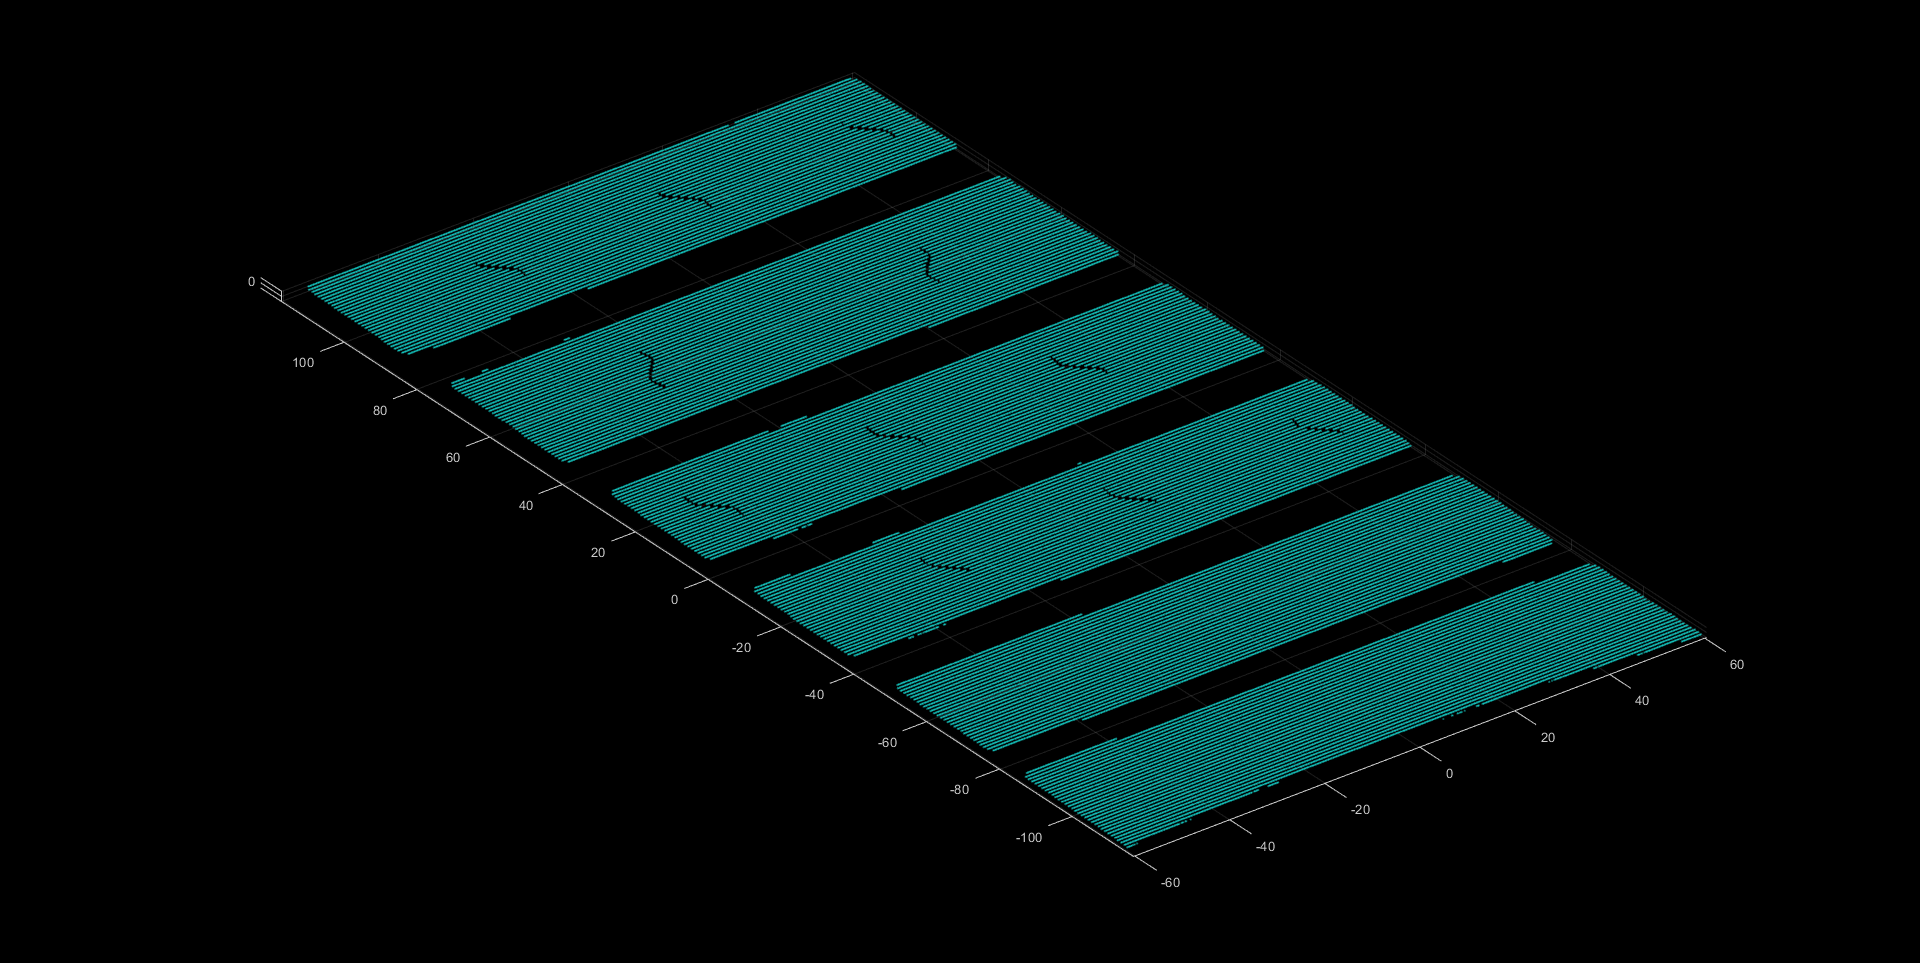
\includegraphics[width=0.45\columnwidth]{./pictures/batt_1b_analisi_2_4.png}
	\caption{Point cloud del battistrada di tipo \textit{1B} dopo aver applicato l'operazione di proiezione.}\label{fig:batt_1b_analisi_4}
\end{figure}

\begin{figure}[H]
	\centering
	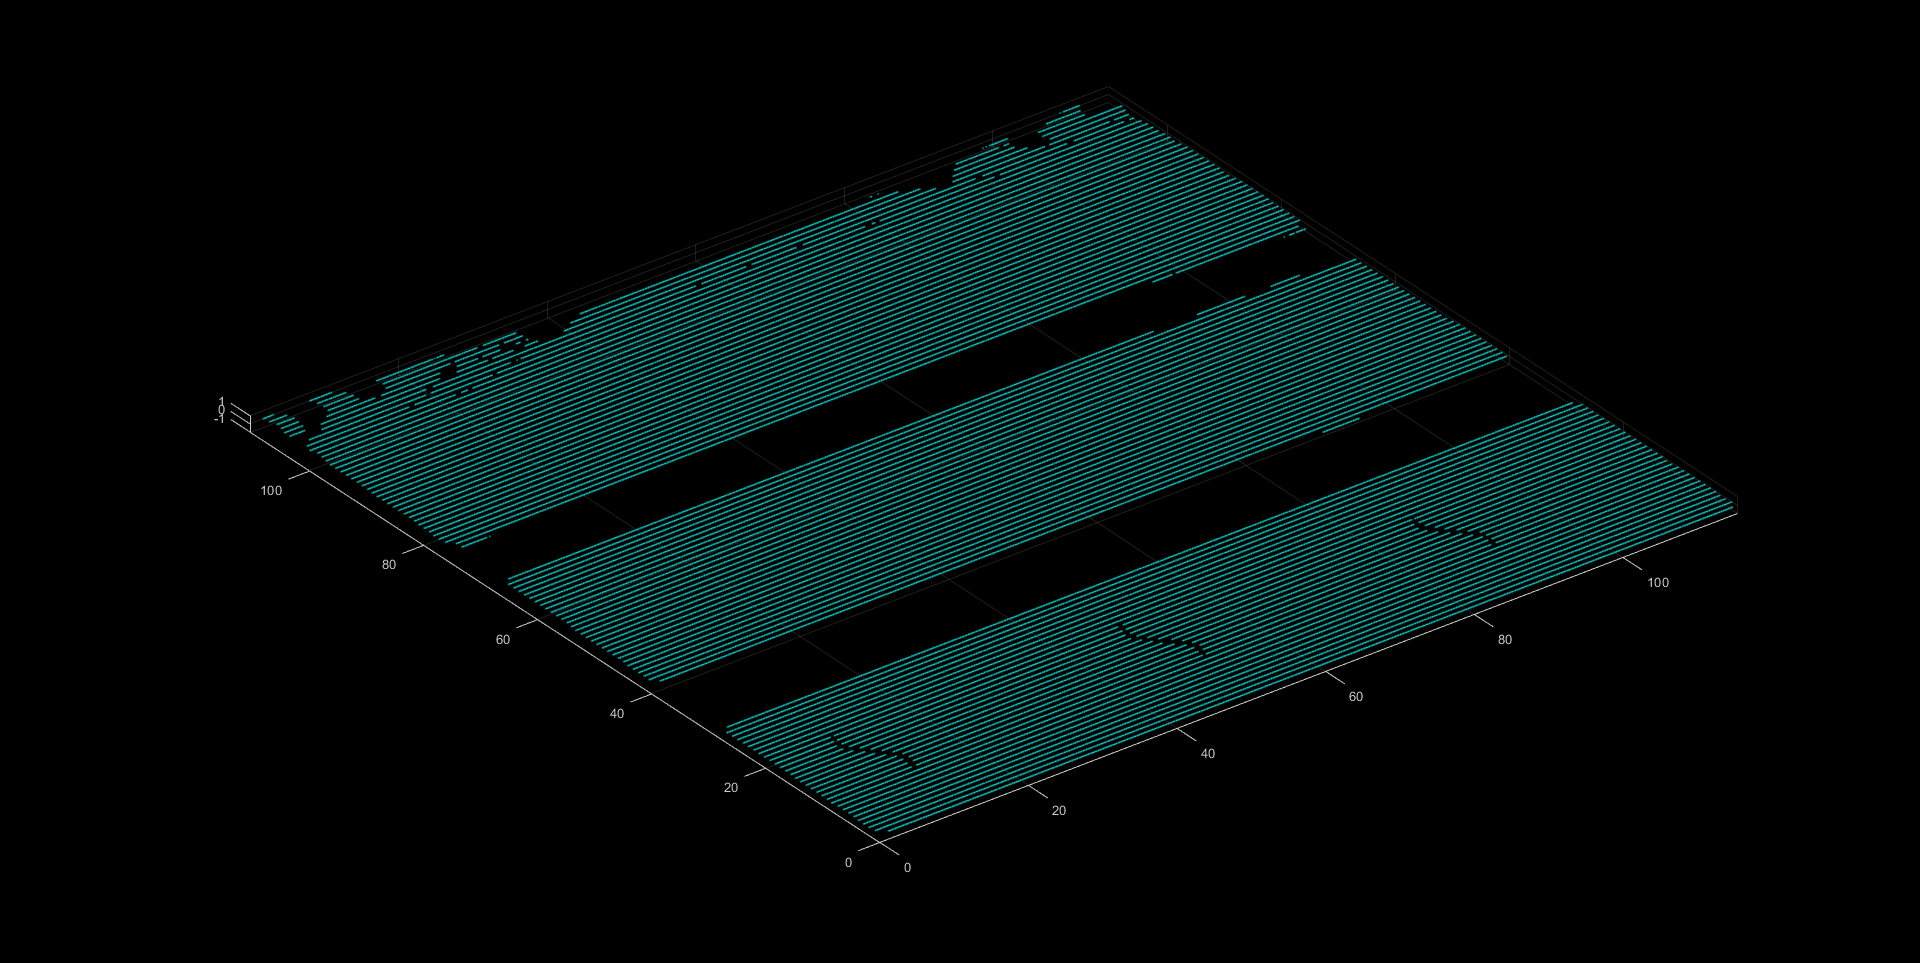
\includegraphics[width=0.45\columnwidth]{./pictures/batt_1b_analisi_1_5.png}
	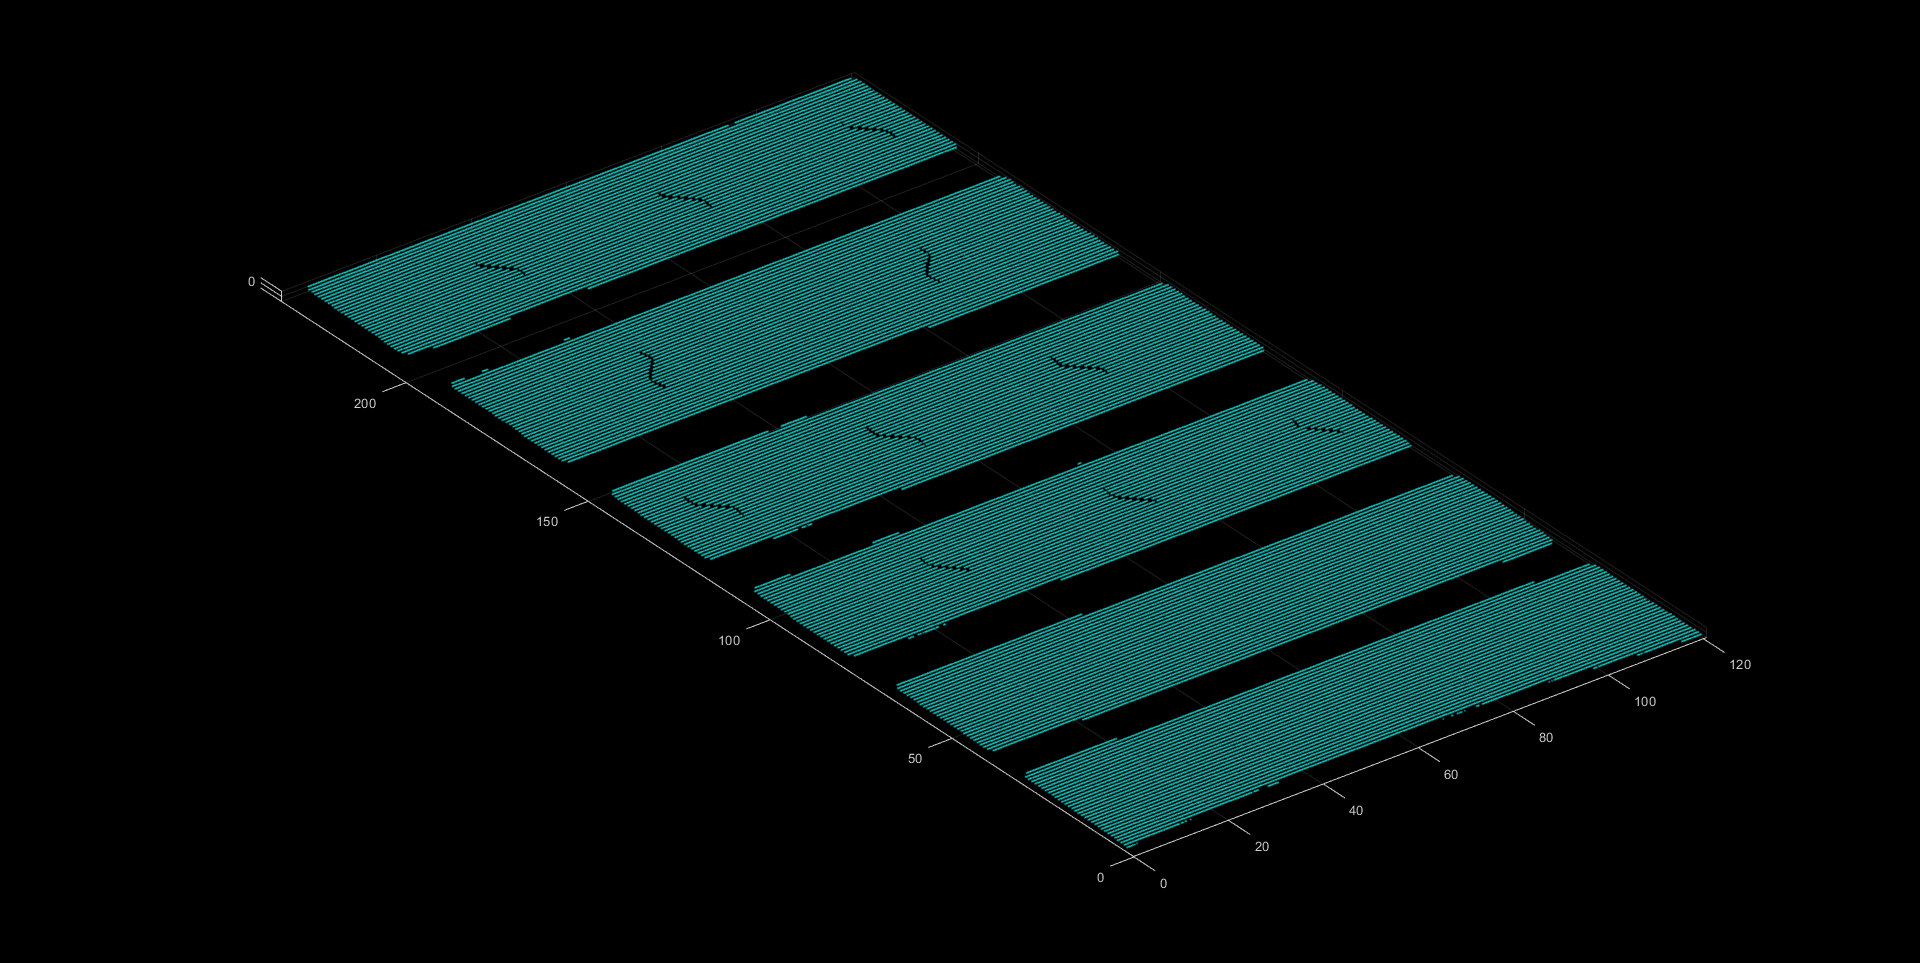
\includegraphics[width=0.45\columnwidth]{./pictures/batt_1b_analisi_2_5.png}
	\caption{Point cloud del battistrada di tipo \textit{1B} dopo aver applicato l'operazione di traslazione.}\label{fig:batt_1b_analisi_5}
\end{figure}

\begin{figure}[H]
	\centering
	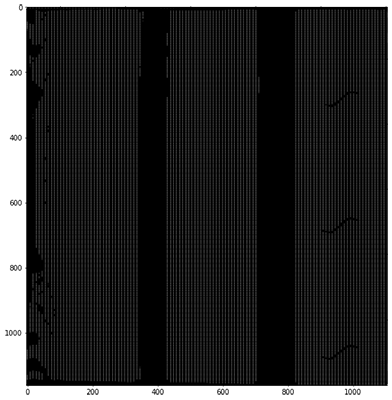
\includegraphics[height=0.32\columnwidth]{./pictures/batt_1b_analisi_1_6.png}
	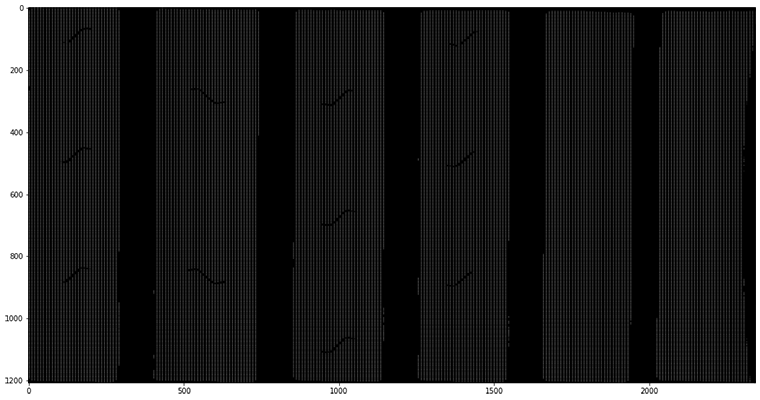
\includegraphics[height=0.32\columnwidth]{./pictures/batt_1b_analisi_2_6.png}
	\caption{Immagine planare del battistrada di tipo \textit{1B}.}\label{fig:batt_1b_analisi_6}
\end{figure}

\begin{figure}[H]
	\centering
	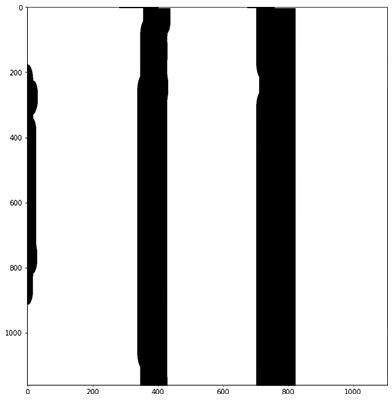
\includegraphics[height=0.32\columnwidth]{./pictures/batt_1b_analisi_1_7.png}
	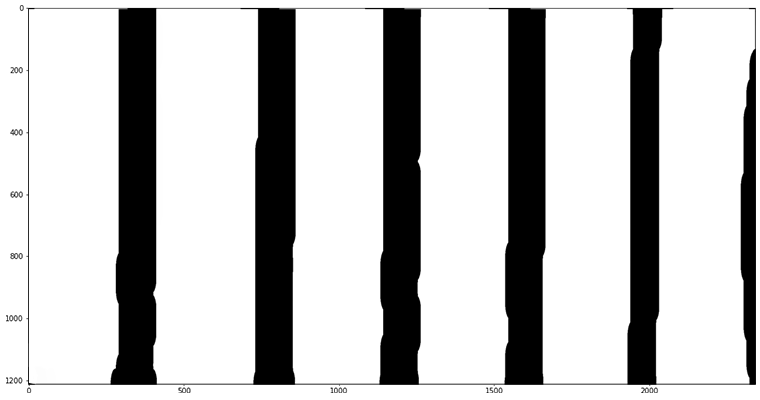
\includegraphics[height=0.32\columnwidth]{./pictures/batt_1b_analisi_2_7.png}
	\caption{Immagine del battistrada di tipo \textit{1B} dopo aver applicato la trasformazione morfologica (Closing).}\label{fig:batt_1b_analisi_7}
\end{figure}

\begin{figure}[H]
	\centering
	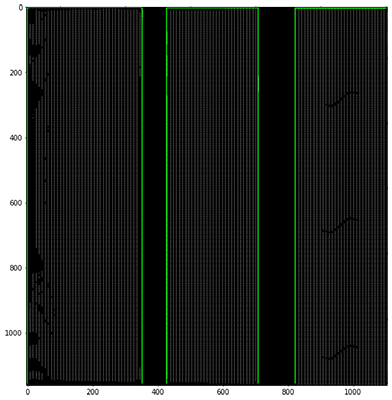
\includegraphics[height=0.32\columnwidth]{./pictures/batt_1b_analisi_1_8.png}
	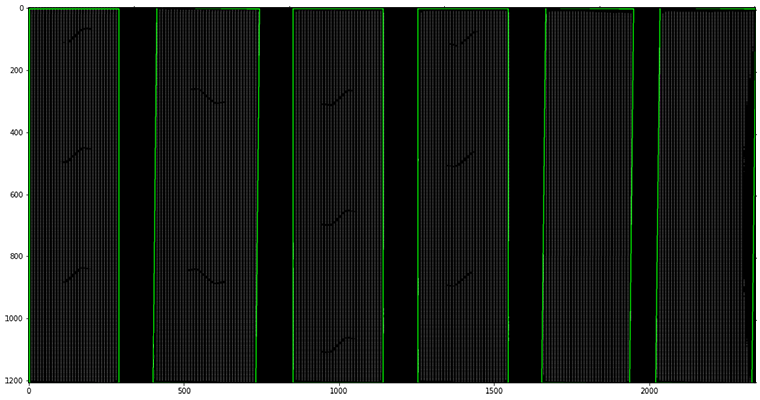
\includegraphics[height=0.32\columnwidth]{./pictures/batt_1b_analisi_2_8.png}
	\caption{Immagine del battistrada di tipo \textit{1B} con le bounding box dei MacroBlob evidenziate.}\label{fig:batt_1b_analisi_8}
\end{figure}


\subsection{Battistrada di tipo 2}
L'analisi di questo tipo di battistrada ha l'obiettivo di estrarre le seguenti features:
\begin{itemize}
	\item Misura della profondità delle scalanature presenti.
	\item Valore minimo, massimo e medio delle profondità.
\end{itemize}

\noindent Come per i battistrada precedenti, in seguito alla scansione dell'oggetto, anche in questo caso viene generata una \textit{point cloud} (figura \ref{fig:batt_2_analisi_1}).\\

\begin{figure}[H]
	\centering
	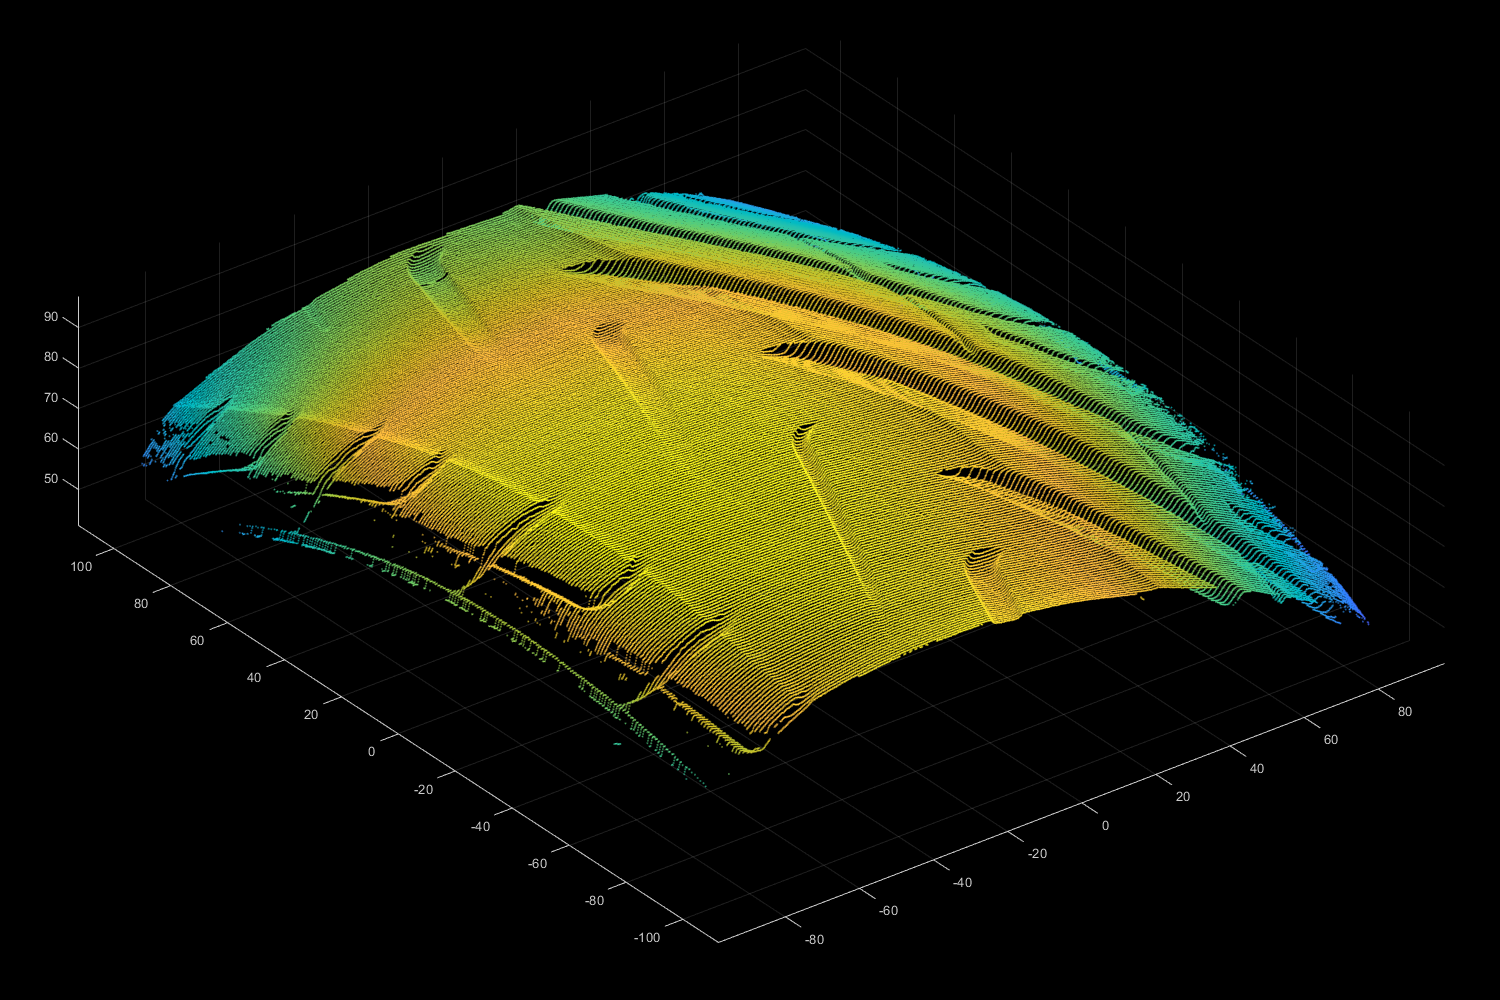
\includegraphics[width=0.45\columnwidth]{./pictures/batt_2_analisi_1.png}
	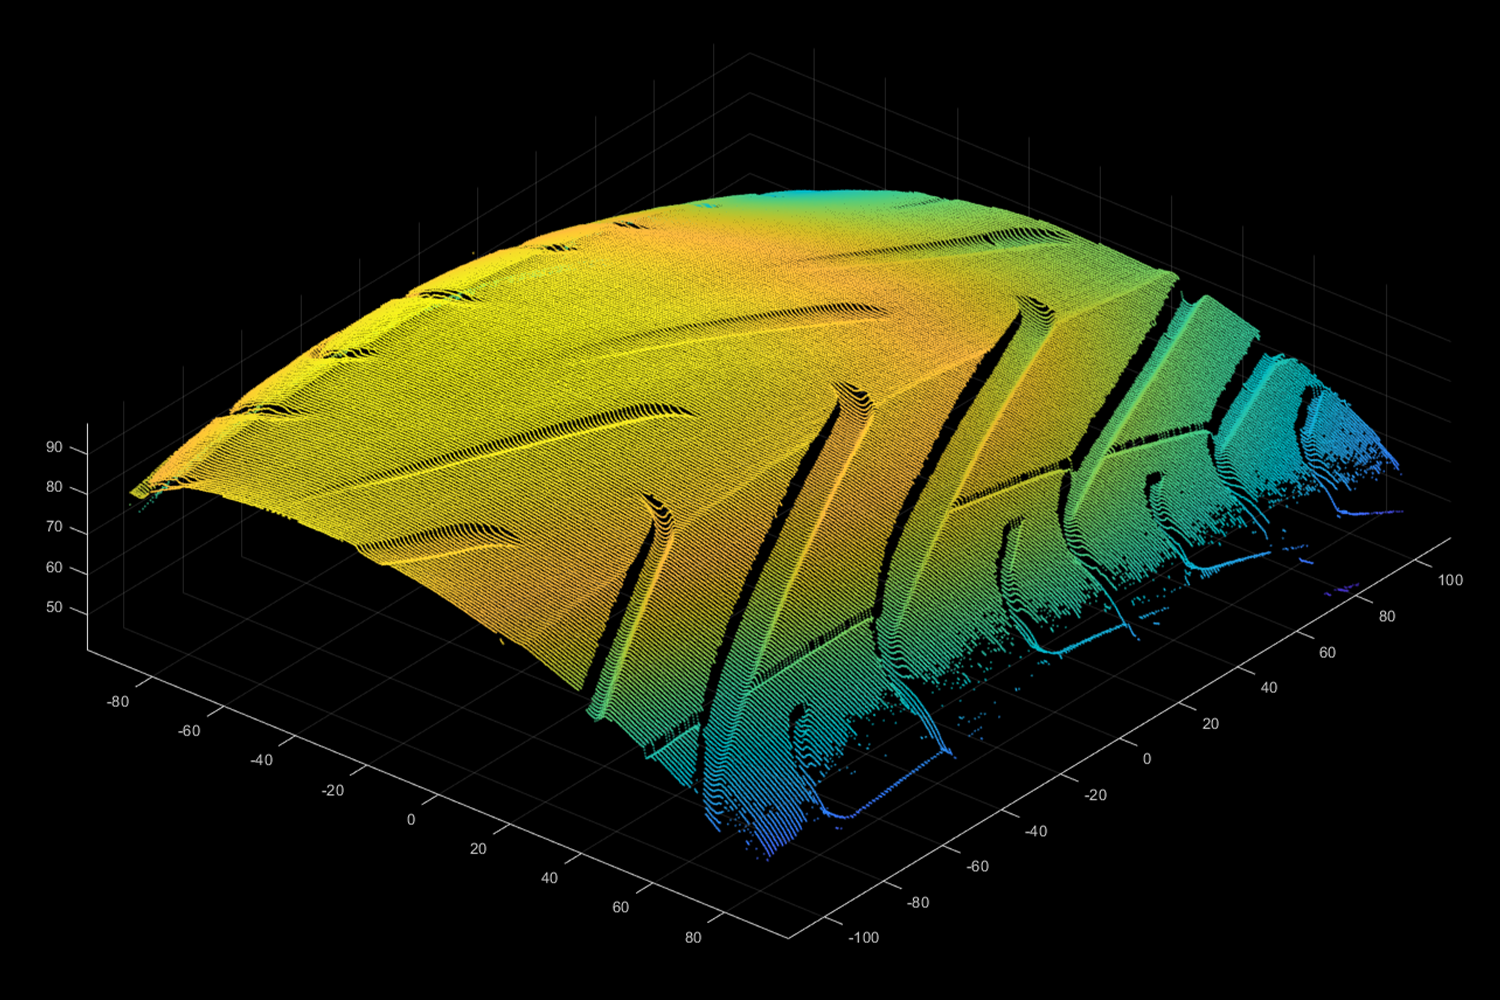
\includegraphics[width=0.45\columnwidth]{./pictures/batt_2_analisi_2.png}
	\caption{Point cloud non elaborata del battistrada di tipo \textit{2}.}\label{fig:batt_2_analisi_1}
\end{figure}

\noindent Per determinare la profondità del battistrada del pneumatico in modo accurato e automatico, è stato sviluppato un metodo di misurazione che prima identifica la posizione delle scanalature e poi calcola, in successione, le profondità di ciascun solco.\\
\newline
L'approccio che si è seguito è quello di scansionare l'intera \textit{point cloud} lungo l'asse \textit{y}, linea per linea, in modo da avere \textit{n} funzioni polinomiali che concatenate ricreino l'intera \textit{point cloud}.\\

\begin{figure}[H]
	\centering
	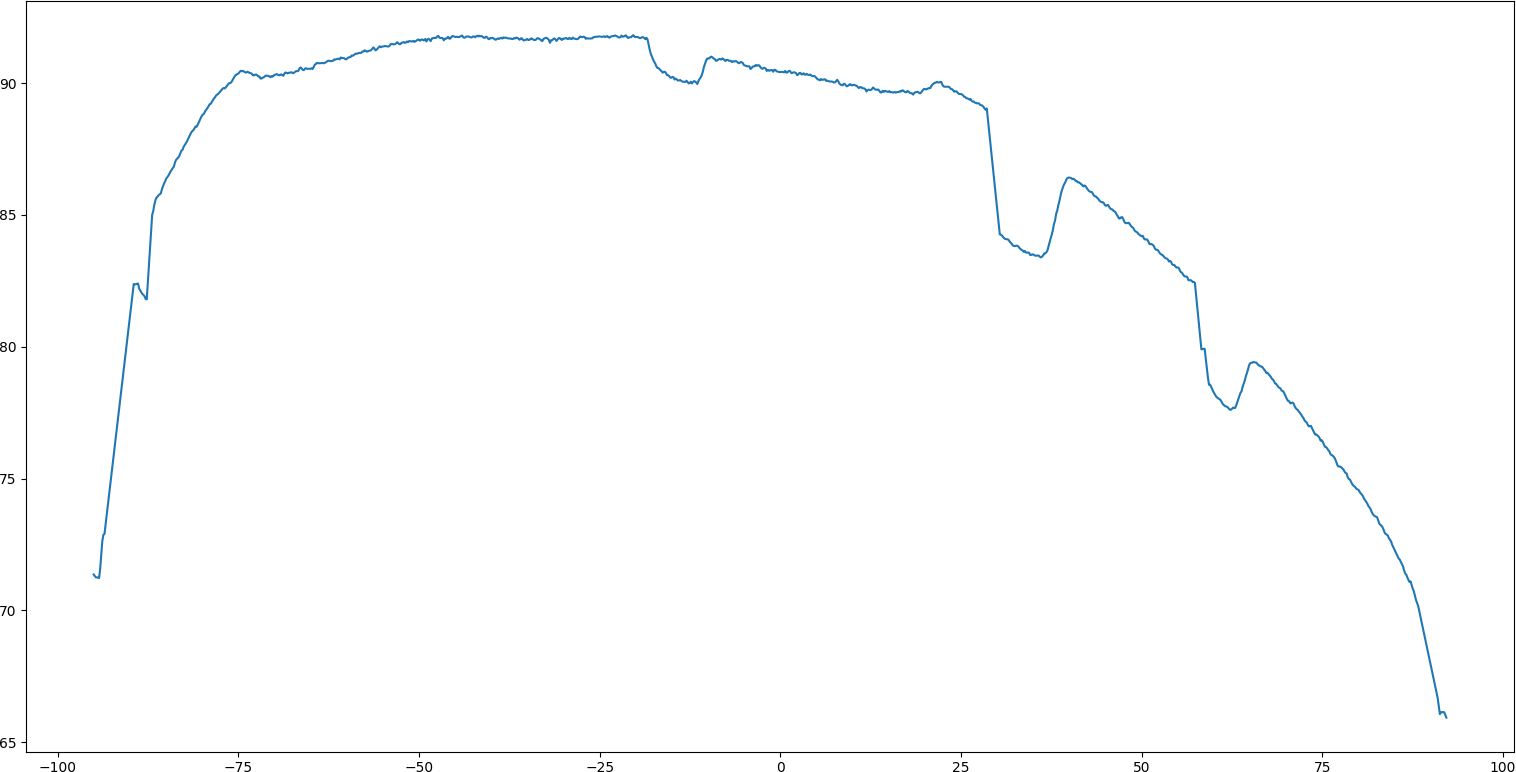
\includegraphics[width=0.9\columnwidth]{./pictures/batt_2_analisi_3.png}
	\caption{Funzione originale.}\label{fig:batt_2_analisi_3}
\end{figure}

\begin{figure}[H]
	\centering
	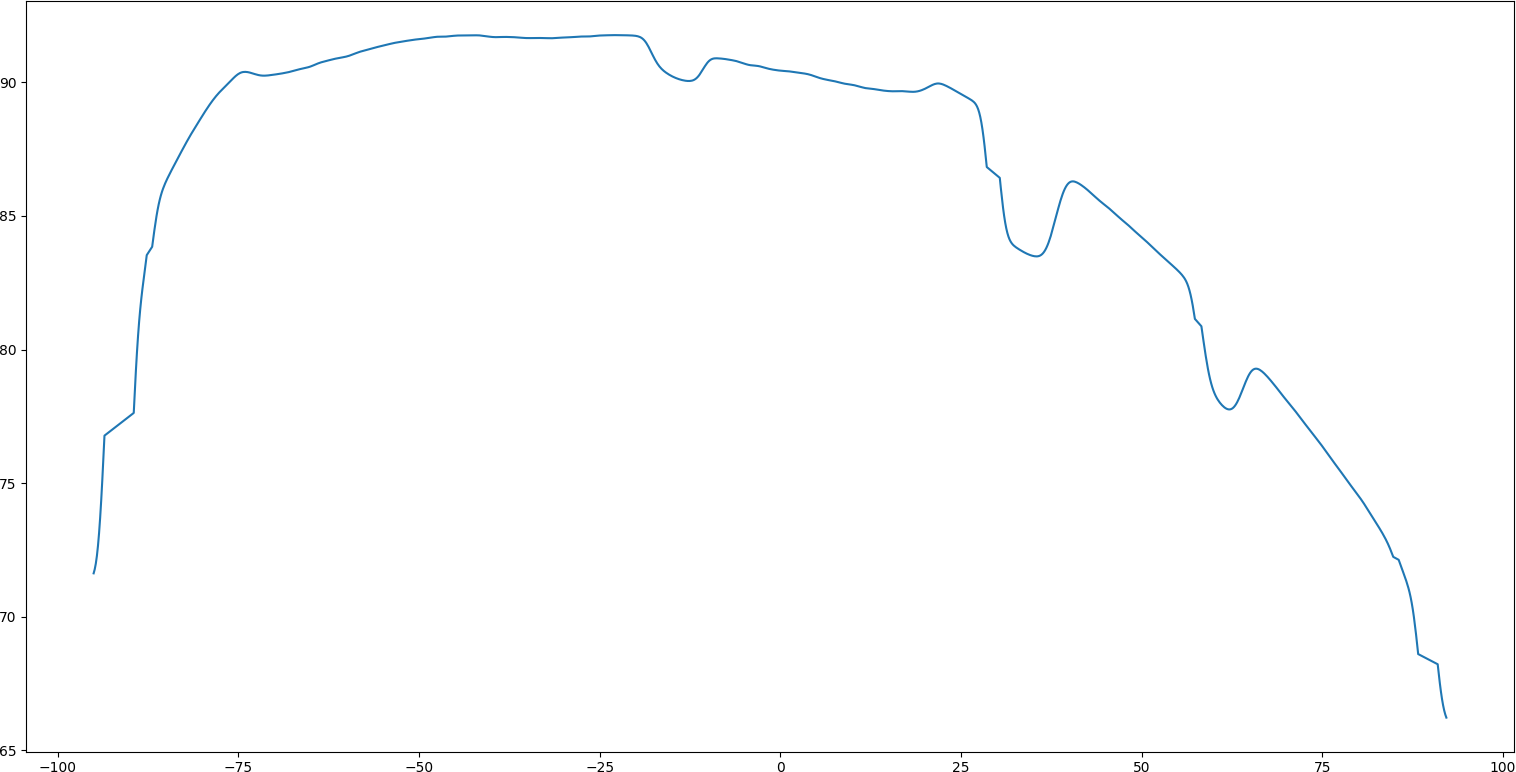
\includegraphics[width=0.9\columnwidth]{./pictures/batt_2_analisi_4.png}
	\caption{Funzione smussata.}\label{fig:batt_2_analisi_4}
\end{figure}

\noindent Per spiegare l'algoritmo prendiamo come esempio una delle \textit{n} funzioni processate. Come si può notare dalla figura \ref{fig:batt_2_analisi_3}, oltre alle scanalature di grandi dimensioni presenti sulla superficie del pneumatico, sono presenti scanalature molto piccole (dovute alla rumorosità) che potrebbero trarre in inganno l'algoritmo di ricerca.\\
\newline
Le scanalature più piccole possono essere rimosse dalla curva del profilo applicando un filtro gaussiano, in modo da rendere la funzione  più smussata (figura \ref{fig:batt_2_analisi_4}). Dopo una serie di prove, come parametri del filtro, sono stati scelti una finestra \textit{$K$ = 51} (dimensione del kernel) e un \textit{$\alpha$ = 5} che specifica il numero di deviazioni standard $\sigma$ desiderate nel kernel.\\
\newline
Ora che la funzione originale è stata smussata, per trovare la posizione e la misura della profondità delle scanalature, ci viene in soccorso lo studio della derivata e dei punti di flesso.\\
\newline
Infatti, tra due punti di massimo della funzione smussata (figura \ref{fig:batt_2_analisi_5}), si trova obbligatoriamente una scanalatura del battistrada, e la profondità di ciascuna scanalatura è data dalla massima distanza che va dal fondo concavo, alla linea che congiunge i due punti di massimo.\\
\newline
Una volta trovati i punti critici nella funzione smussata, sono state salvate le rispettive coordinate \textit{x} di ogni punto e riportate nella funzione originale (figura \ref{fig:batt_2_analisi_6} e figura \ref{fig:batt_2_analisi_7}).\\

\begin{figure}[H]
	\centering
	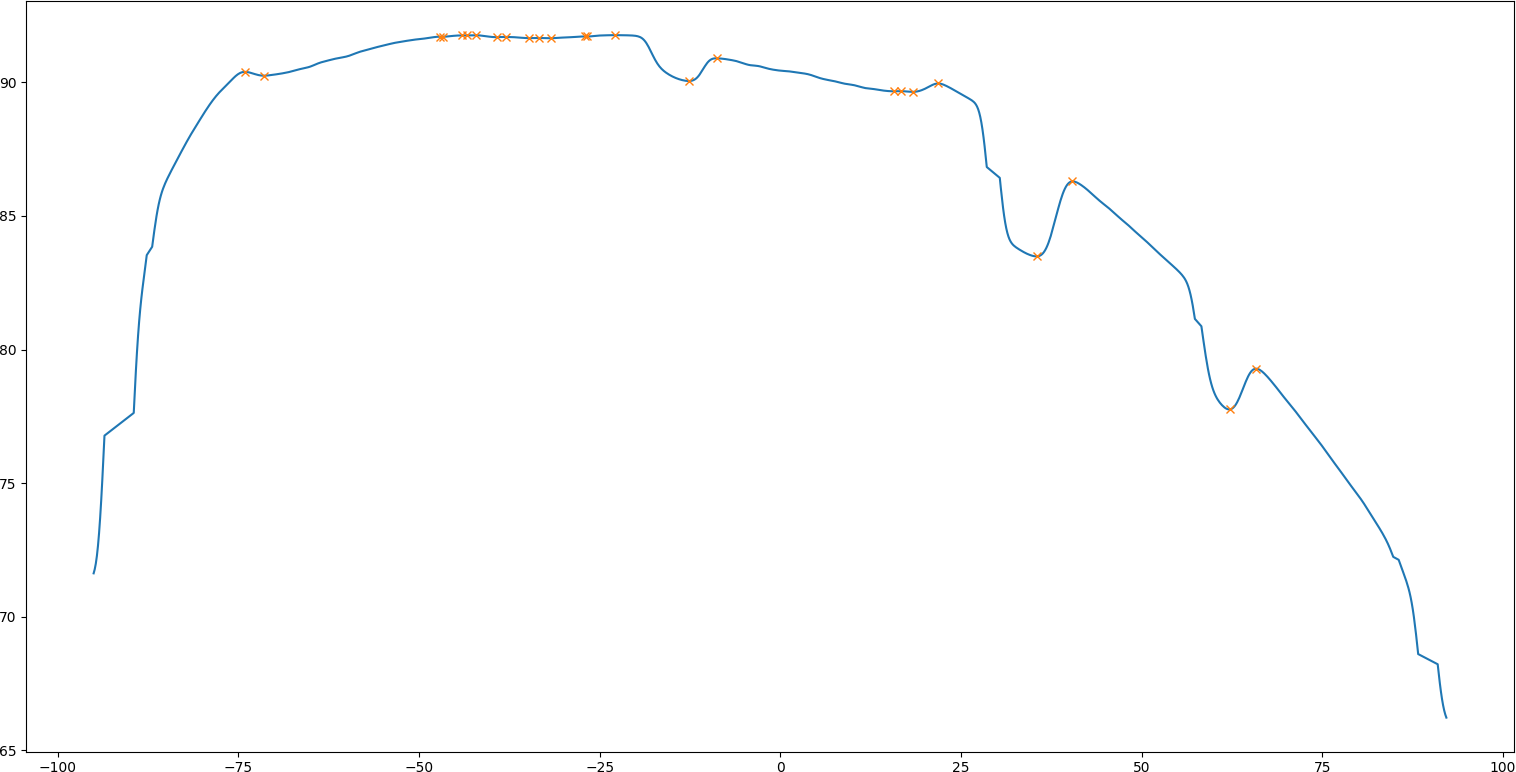
\includegraphics[width=0.9\columnwidth]{./pictures/batt_2_analisi_5.png}
	\caption{Massimi e minimi della funzione smussata.}\label{fig:batt_2_analisi_5}
\end{figure}

\begin{figure}[H]
	\centering
	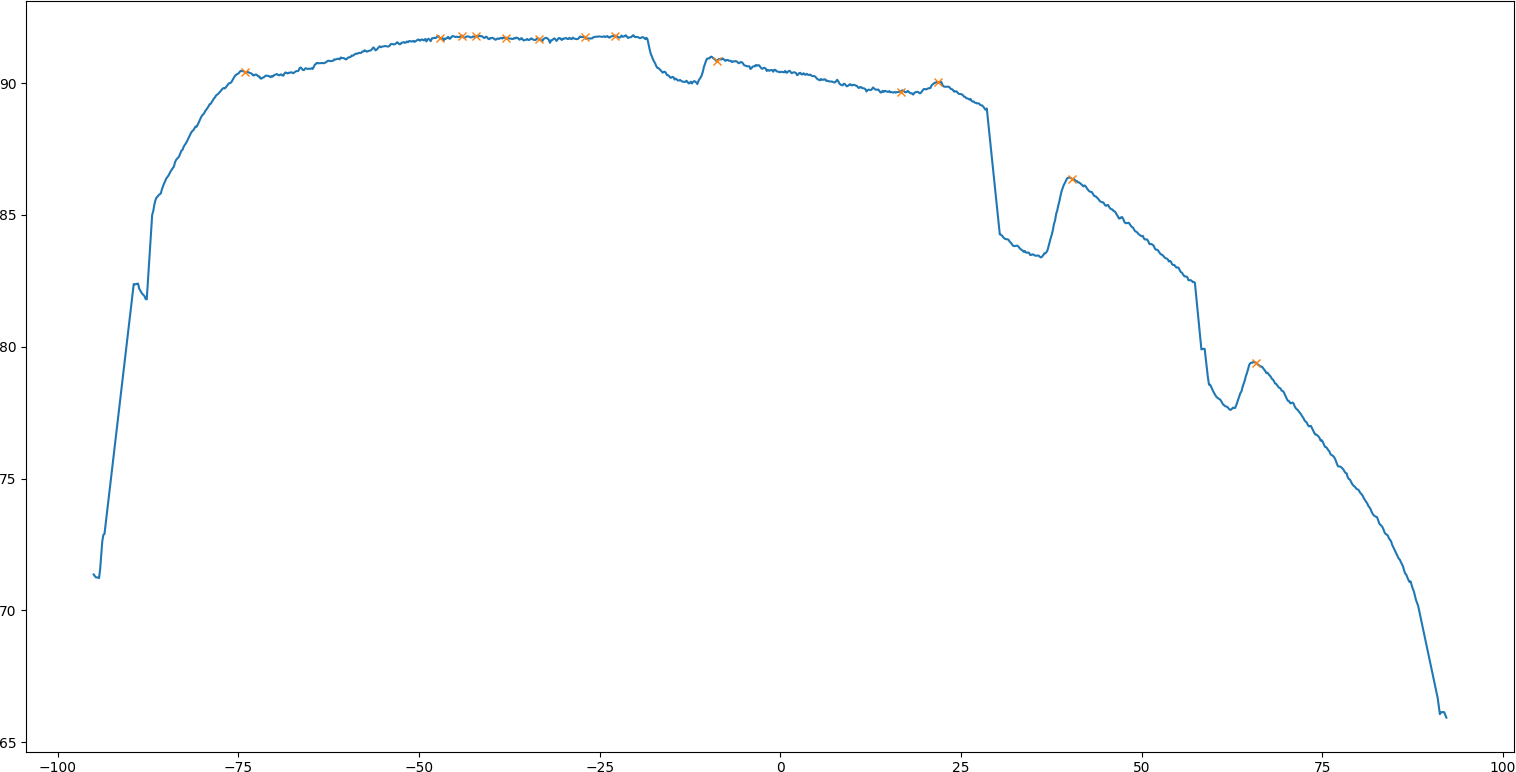
\includegraphics[width=0.9\columnwidth]{./pictures/batt_2_analisi_6.png}
	\caption{Massimi (da destra) della funzione originale.}\label{fig:batt_2_analisi_6}
\end{figure}

\begin{figure}[H]
	\centering
	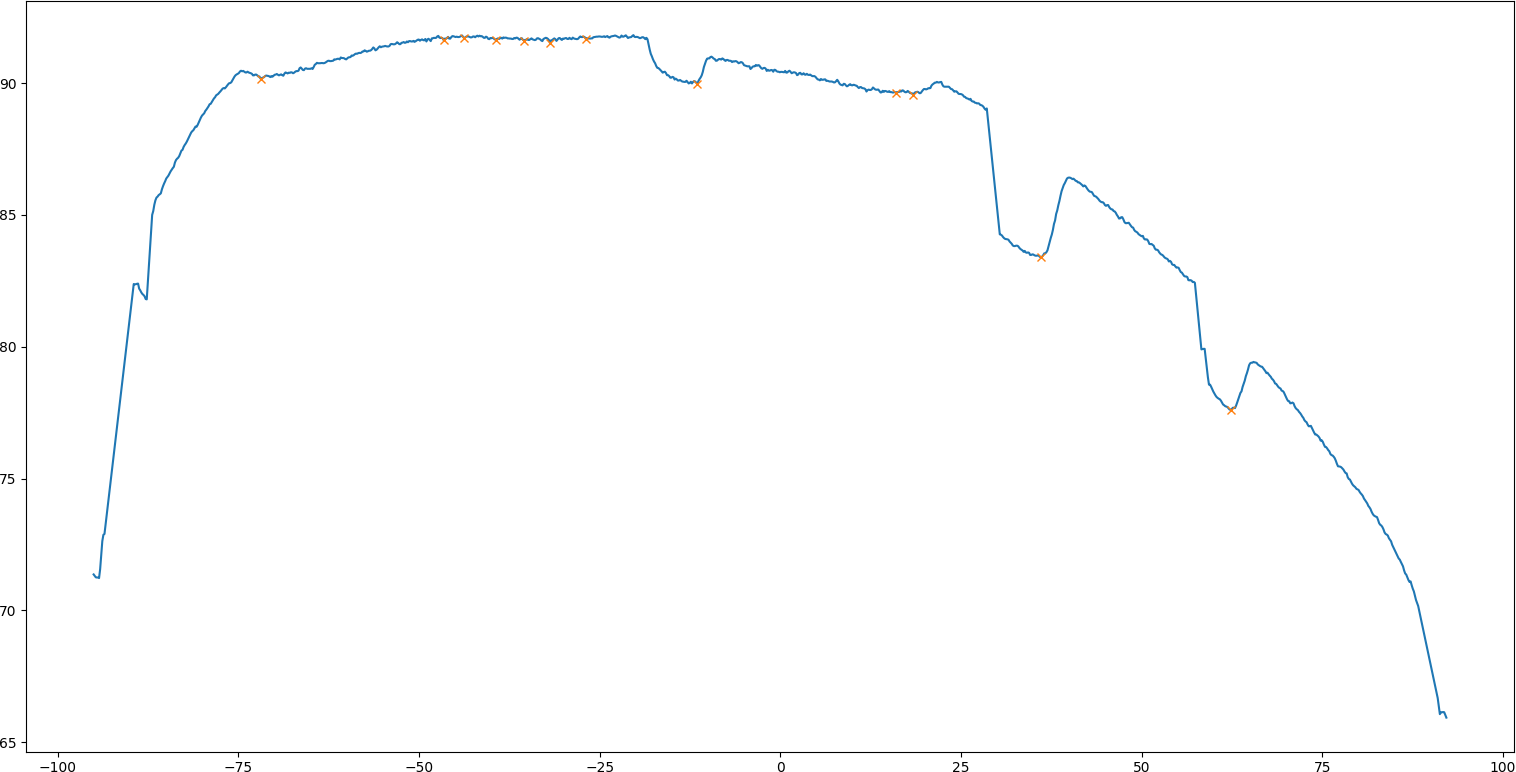
\includegraphics[width=0.9\columnwidth]{./pictures/batt_2_analisi_7.png}
	\caption{Minimi della funzione originale.}\label{fig:batt_2_analisi_7}
\end{figure}

\noindent Seguendo il percorso del profilo del battistrada, a partire dall'estrema destra, ciò che abbiamo trovato fino ad ora sono: il punto dove inizia la scanalatura, il punto più profondo di essa e il punto dove inizia l'eventuale scanalatura successiva.\\
\newline
Quindi, per migliorare la precisione della posizione delle scanalature, dobbiamo trovare la posizione del punto di chiusura di ogni scanalatura.
\newpage
\noindent Per trovare questi punti, che chiameremo impropriamente punti di massimo da sinistra, si è seguito il seguente algoritmo:

\begin{itemize}
	\item Isolare la parte di funzione che si trova tra un minimo e il massimo successivo;
	\item Ruotarla, facendo in modo che la retta passante tra il minimo e il massimo sia parallela all'asse delle \textit{x};
	\item Individuare il punto di massimo della porzione di funzione ruotata, che in definitiva sarà il nostro massimo da sinistra;
\end{itemize}

\noindent Così facendo si trova un buon punto di massimo approssimato, dato che la rotazione non intacca la posizione dei punti.\\
\newline
Nella figura \ref{fig:batt_2_analisi_8} è illustrato un esempio di questo calcolo, con evidenziate di verde, sia la funzione smussata sia quella ruotata, da cui si è individuato il nostro punto di massimo.\\
\newline
Una volta ripetuto l'algoritmo per ogni tratto della funzione smussata, la posizione di ogni punto di massimo trovata, è stata riportata nella funzione originale (figura \ref{fig:batt_2_analisi_9}).\\

\begin{figure}[H]
	\centering
	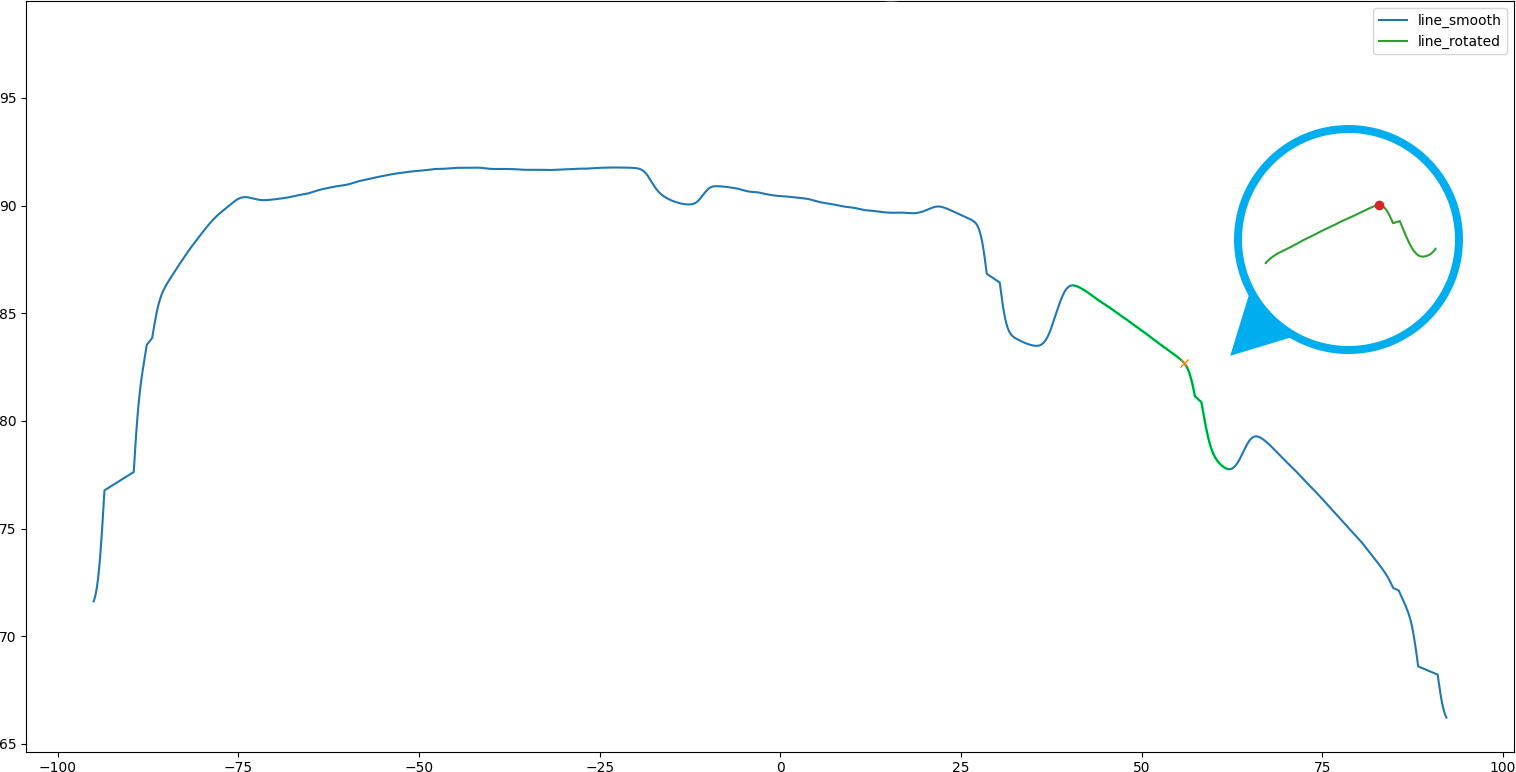
\includegraphics[width=0.9\columnwidth]{./pictures/batt_2_analisi_8.png}
	\caption{Esempio del calcolo di uno dei massimi (da sinistra) della funzione smussata.}\label{fig:batt_2_analisi_8}
\end{figure}

\begin{figure}[H]
	\centering
	\includegraphics[width=0.9\columnwidth]{./pictures/batt_2_analisi_9.png}
	\caption{Massimi (da sinistra) della funzione originale.}\label{fig:batt_2_analisi_9}
\end{figure}

\noindent Dopo aver chiarito definitivamente la posizione e il numero delle scanalature del battistrada, è possibile misurare la profondità di ciascuna scanalatura, calcolando la distanza tra la retta che congiunge un massimo da destra e un massimo da sinistra, e il punto di minimo corrispondente.\\
\newline
In fine è stato applicato un filtro, in modo tale da prendere solo le distanze che siano maggiori di 0.5 millimetri (figura \ref{fig:batt_2_analisi_10}).\\

\begin{figure}[H]
	\centering
	\includegraphics[width=0.9\columnwidth]{./pictures/batt_2_analisi_10.png}
	\caption{Confronto tra la funzione originale e la funzione smussata. I punti critici segnati sono il risultato di un filtro sulla distanza maggiore di 0.5 millimetri.}\label{fig:batt_2_analisi_10}
\end{figure}

\begin{figure}[H]
	\centering
	\includegraphics[width=0.5\columnwidth]{./pictures/battistrada.png}
	\caption{Point cloud del battistrada di tipo \textit{2}, con vista sul piano \textit{XY}.}\label{fig:battistrada}
\end{figure}

\begin{figure}[H]
	\centering
	\subfloat[][]{\includegraphics[height=0.6\columnwidth]{./pictures/battistrada_maxr_maxl_0.3.png}}
	\hspace{1em}
	\subfloat[][]{\includegraphics[height=0.6\columnwidth]{./pictures/battistrada_maxr_min_maxl_0.3.png}}
	\caption{(a) Point cloud contenente i punti di massimo da sinistra e di massimo da destra. (b) Point cloud contenente i punti di minimo, massimo da sinistra e di massimo da destra.}\label{fig:battistrada_maxr_maxl_0.3}
\end{figure}
\cleardoublepage
\chapter{Applicazione desktop}
\label{Cha:desktop}
\thispagestyle{empty}

Il capitolo seguente sarà incentrato sulla presentazione dell'applicazione desktop e delle sue interfacce e funzionalità.

\section{Sviluppo}
L'applicazione è stata creata su \textit{Visual Studio}, utilizzando il framework \textit{WPF} (Windows Presentation Foundation) che fornisce agli sviluppatori un modello di programmazione unificato per la creazione di applicazioni client desktop.\\
\newline
La piattaforma di sviluppo \textit{WPF} supporta un'ampia serie di funzionalità di sviluppo di applicazioni, inclusi un modello applicativo, risorse, controlli, elementi grafici, layout, data binding, documenti e sicurezza.\\
\newline
La parte di \textit{setup} con il Gocator e l'implementazione degli algoritmi di analisi sono stati esportati in una \textit{DLL} (dynamic-link library) che è una libreria a collegamento dinamico che contiene codice e dati che possono essere usati da più programmi contemporaneamente.\\
\newline
In seguito, il collegamento tra la libreria \textit{DLL} e il codice dell'interfaccia grafica, è stato effettuato eseguendo il wrapping di una classe \textit{C++}, contenente le funzioni da esportare, in modo tale da essere usate dal codice creato in \textit{C\#}.\\
\newline
Sono state utilizzate anche le \textit{named pipe}, che forniscono la comunicazione interprocesso tra un server pipe e uno o più client pipe.

\section{Librerie di supporto}
Le librerie utilizzate per realizzare l'applicazione grafica sono:

\begin{itemize}
	\item \textit{JSON for Modern C++, versione 3.10.5}, è una libreria per elaborare dati in formato \textit{JSON};
	\item \textit{Helix Toolkit, versione 2.20.2}, è una raccolta di componenti 3D per \textit{.NET};
	\item \textit{Json.NET - Newtonsoft, versione 13.0.1}, è un popolare framework JSON ad alte prestazioni per \textit{.NET};
	\item \textit{Ookii.Dialogs.Wpf, versione 5.0.1}, è una libreria per applicazioni \textit{WPF}.
\end{itemize}

\section{Interfaccia grafica}
L'interfaccia grafica è stata pensata per essere semplice e intuitiva. È presente un pannello di configurazione, uno dove vengono stampati a video i dati derivati dall'analisi e una sezione dove si può visualizzare e interagire con la \textit{point cloud}.

\begin{figure}[H]
	\centering
	\includegraphics[width=1.0\columnwidth]{./pictures/gui_1.png}
	\caption{Interfaccia grafica con la descrizione dei pulsanti.}\label{fig:gui_1}
\end{figure}

\noindent Di seguito la descrizione dei pulsanti:

\begin{itemize}
	\item \textbf{1:} Connette e disconnette il sensore, tramite indirizzo IP;
	\item \textbf{2:} Aggiorna il valore dell'esposizione;
	\item \textbf{3:} Carica il file in formato \textit{.pcd} della \textit{point cloud} del battistrada;
	\item \textbf{4:} Seleziona il tipo di battistrada da analizzare;
	\item \textbf{5:} Seleziona la cartella dove salvare le \textit{point cloud}, create durante l'analisi;
	\item \textbf{6:} Visualizzatore 3D delle \textit{point cloud};
	\item \textbf{7:} Seleziona le \textit{point cloud} da visualizzare per oggetto scansionato;
	\item \textbf{8:} Scorre indietro le \textit{point cloud};
	\item \textbf{9:} Scorre avanti le \textit{point cloud};
	\item \textbf{10:} Resetta la visualizzazione e rimuove le \textit{point cloud} caricate;
	\item \textbf{11:} Avvia l'acquisizione dal Gocator;
	\item \textbf{12:} Interrompe l'acquisizione dal Gocator;
	\item \textbf{13:} Avvia l'analisi offline del file caricato;
\end{itemize}

\noindent Quindi, il programma può essere utilizzato sia in modalità online (connesso direttamente al Gocator) sia in modalità offline (caricando e analizzando il file della \textit{point cloud} del battistrada).\\
\newline
La modalità online permette di:

\begin{itemize}
	\item Inserire l'indirizzo IP del sensore, connettersi e disconnettersi;
	\item Modificare il valore dell'esposizione;
	\item Selezionare il tipo di battistrada da analizzare;
	\item Salvare i file in formato \textit{.pcd}, durante l'analisi, delle \textit{point cloud} step by step;
	\item Avviare e stoppare la scansione, con la visualizzazione del risultato dell'analisi in real time;
	\item Visualizzare a video le \textit{point cloud} dei battistrada scansionati e analizzati;
\end{itemize}

\noindent La modalità offline permette di:

\begin{itemize}
	\item Caricare un file contenente la \textit{point cloud} del battistrada;
	\item Selezionare il tipo di battistrada da analizzare;
	\item Salvare, durante l'analisi, le \textit{point cloud} step by step;
	\item Avviare l'analisi del file;
	\item Visualizzare a video le \textit{point cloud} caricate;
\end{itemize}

\begin{figure}[H]
	\centering
	\includegraphics[width=0.9\columnwidth]{./pictures/gui_3.png}
	\caption{Interfaccia grafica con la point cloud filtrata visualizzata a video.}\label{fig:gui_2}
\end{figure}

\noindent In particolare, nel caso del battistrada di tipo \textit{2}, il risultato della scansione riporta a video, oltre alla \textit{point cloud} del battistrada, anche la stessa con evidenziati i punti di altezza delle scanalature minima e massima, e la \textit{point cloud} con solo i punti di massimo da sinistra e destra (figura \ref{fig:gui_4}, figura \ref{fig:gui_5} e figura \ref{fig:gui_6}).

\begin{figure}[H]
	\centering
	\includegraphics[width=0.9\columnwidth]{./pictures/gui_4.png}
	\caption{Interfaccia grafica con, visualizzata a video, la point cloud del battistrada di tipo 1A e il risultato dell'analisi.}\label{fig:gui_3}
\end{figure}

\begin{figure}[H]
	\centering
	\includegraphics[width=0.9\columnwidth]{./pictures/gui_5.png}
	\caption{Interfaccia grafica con, visualizzata a video, la point cloud del battistrada di tipo 2.}\label{fig:gui_4}
\end{figure}

\begin{figure}[H]
	\centering
	\includegraphics[width=0.9\columnwidth]{./pictures/gui_6.png}
	\caption{Interfaccia grafica con, visualizzata a video, la point cloud con i punti di profondità delle scanalature minima e massima.}\label{fig:gui_5}
\end{figure}

\begin{figure}[H]
	\centering
	\includegraphics[width=0.9\columnwidth]{./pictures/gui_7.png}
	\caption{Interfaccia grafica con, visualizzata a video, la point cloud filtrata.}\label{fig:gui_6}
\end{figure}
\cleardoublepage
\chapter{Conclusioni}
\label{Cha:conclusioni}
\thispagestyle{empty}

L'ultimo capitolo fornisce una sintesi dei risultati ottenuti e alcuni suggerimenti su possibili problematiche che potrebbero essere risolte in futuro.

\section{Risultati ottenuti}
I risultati sperimentali hanno rilevato che il sistema è in grado di acquisire correttamente le \textit{point cloud} dei battistrada e che gli algoritmi possono effettuare misurazioni, identificare le scanalature e misurarne la profondità.\\
\newline
Riprendendo i test effettuati nel paragrafo \ref{performance}, riportiamo i risultati delle scansioni riguardante il battistrada di tipo \textit{2}:

\begin{table}[H]
\centering
\begin{tabular}{||c c c c||} 
 \hline
 N & min (mm) & max (mm) & avg (mm) \\ [0.5ex]
 \hline\hline
 1 & 0.50 & 4.85 & 2.68 \\ 
 \hline
 2 & 0.50 & 4.73 & 2.62 \\
 \hline
 3 & 0.51 & 4.76 & 2.64 \\
 \hline
 4 & 0.51 & 4.80 & 2.66 \\
 \hline
 5 & 0.50 & 4.85 & 2.68 \\
 \hline
 6 & 0.50 & 4.77 & 2.64 \\
 \hline
 7 & 0.51 & 4.82 & 2.67 \\
 \hline
 8 & 0.50 & 4.82 & 2.66 \\
 \hline
 9 & 0.50 & 4.79 & 2.65 \\
 \hline
 10 & 0.51 & 4.80 & 2.66 \\
 \hline
\end{tabular}
\caption{Valori calcolati su una serie di misurazioni del battistrada di tipo 2.}
\label{table:1}
\end{table}

\noindent Ogni misura calcolata dal programma è stata verificata direttamente sugli pneumatici utilizzando un calibro. Nonostante il punto di profondità massima cambiasse leggermente posizione, le misurazioni sono risultate abbastanza accurate e i test hanno sancito il raggiungimento dell'obiettivo che ci si era posti per il progetto.\\

\begin{figure}[H]
	\centering
	\includegraphics[width=0.40\columnwidth]{./pictures/gocator_conveyor_1.jpg}
	\hspace{1em}
	\includegraphics[width=0.40\columnwidth]{./pictures/gocator_conveyor_2.jpg}
	\caption{Il Gocator in azione durante una scansione.}\label{fig:gocator_conveyor}
\end{figure}

\section{Conclusione e lavori futuri}
Grazie allo studio di questa materia e al rispettivo progetto d'esame, è stata esplorata una branca dell'intelligenza artificiale molto importante per la moltitudine di benefici che apporta in tutti i settori per migliorare l'esperienza del consumatore, ridurre i costi e aumentare la sicurezza.\\
\newline
Seppure i risultati ottenuti sono risultati molto buoni, il margine di miglioramento è ampio, ed una futura ottimizzazione degli algoritmi e di altri particolari del Gocator, potrebbe portare a risultati ancora migliori.

\nocite{opencv_library}
\nocite{helix_toolkit_documentation}
\nocite{wpf_whatis}
\nocite{wrapping_whatis}
\nocite{dll_whatis}
\nocite{direct_industry}
\nocite{redazione_geomedia}
\nocite{lmi_technologies}
\nocite{image_s_blog}
\nocite{point_cloud_library_1}
\nocite{point_cloud_library_2}
\nocite{point_cloud_library_3}
\nocite{point_cloud_library_4}
\nocite{the_gsl_team}
\nocite{wang2019}
\nocite{booksdaglib0034531}
\nocite{gonzalez2008digital}
\nocite{named_pipe_whatis}
\cleardoublepage
\appendix


%\include{Appendix}

% ---- Bibliography ----
\addcontentsline{toc}{chapter}{Bibliografia}
\printbibliography
\thispagestyle{empty} \vspace*{.75truecm} \cleardoublepage
%\include{ringraziamenti}
%\thispagestyle{empty} \vspace*{.75truecm} \cleardoublepage


\end{document}